% !TEX root = ../thesis.tex

%
%
%\chapter{The Panoptic Studio: A Massively Multiview Capture System}
%\section{Modularized Hardware Design}
%\subsection{Structure}
%\subsection{Architecture}
%\section{Calibration}
%\subsection{Temporal Calibration}
%\subsection{Spatial Calibration}
%\section{Capture Procedures}
%
%\chapter{Methods For Social Interaction Capture}
%\section{Dense Trajectory Stream Reconstruction}
%\section{Markerless Social Interaction Capture}
%\subsection{Body}
%\subsection{Face}
%\subsection{Hand}
%\section{Motion Refinement to Capture Subtle Details (Proposed)}
%\section{Panoptic Studio Dataset}


\chapter{The Panoptic Studio}%: A Massively Multiview System}
\label{chapter:system}

There are principal challenges in capturing social signals between individuals in a group: (1) social interactions have to be sensed over a volume sufficient to house a dynamic social group, yet subtle details of the motion where important social signals are embedded must be captured; (2) strong occlusions emerge functionally in natural social interactions (e.g., people systematically face each other while interacting, bodies are occluded by gesticulating limbs); (3) human appearance and configuration variation is immense; and (4) social signaling is sensitive to interference---for instance, attaching markers to the face or body, a pre-capture model building stage, or even instructing each individual to assume a canonical body pose during an interaction, primes the nature of subsequent interactions. 

The Panoptic Studio is developed to overcome these challenges. The system has a large geodesic sphere structure with a 5.49m diameter, with heterogeneous sensors on its surface including 480 VGA cameras, 31 HD cameras, 10 RGB+D sensors, 23 microphones, and 5 DLP projectors. The core principle and motivation in building this system is to obtain as much measurement as possible to have minimum assumptions about the scenes. We found that the large number of views of the system greatly relieves all the aforementioned sensing challenges, and also enables us to use relatively ``weak" perceptual processes from the large number of views rather than a complicated method with strong assumptions about the scenes. To this end, this system enables us to measure a broad spectrum of social signals of naturally interacting groups. This chapter covers the various hardware and low-level software issues in building the Panoptic Studio, including structure design, architectures, synchronization, and spatial calibration.  

The Panoptic Studio is the output of several years of collaboration with Tomas Simon, Xulong Li, Hao Liu, Lei Tan, Lin Gui, Timothy Godisart, Sean Banerjee, Hyun Soo Park, Iain Matthews, Bart Nabbe, Shohei Nobuhara, Takeo Kanade, and Yaser Sheikh. 
%do not introduce any kind of sight restriction on the subjects
%Why not using just 100 HD instead of this combination?)
%Modularized design is the key (same number of cameras, HD on the center). 

% Modularized design, VGA, HD, Kinect
\section{Structural Design}
% Add optimization routine
The physical frame of the studio is a variant of a face-transitive solid called a truncated pentagonal hexecontahedron. This particular structure was selected because it has among the largest number of transitive faces of any geodesic dome~\cite{Williams1979}. The transitivity of the faces enables the modular architecture, and ensures that the structure remains easy to upgrade and customize with different panels of the same configuration. The structure has a diameter of 5.49m and a total height of 4.15m. The floor of the dome is 1.40m below the center of the sphere structure to increase access to the edges. In all, the structure consists of 6 pentagonal panels, 40 hexagonal panels, and 10 trimmed base panels. The interior and exterior view of the Panoptic Studio are shown in Figure~\ref{fig:dome_ext_int} and a 360\degree~panoramic view of the interior of the Panoptic Studio is shown in Figure~\ref{fig:dome_panorama}. The structural design is illustrated in the left of Figure~\ref{fig:dome_structure}.


\begin{figure}
	\centering       
	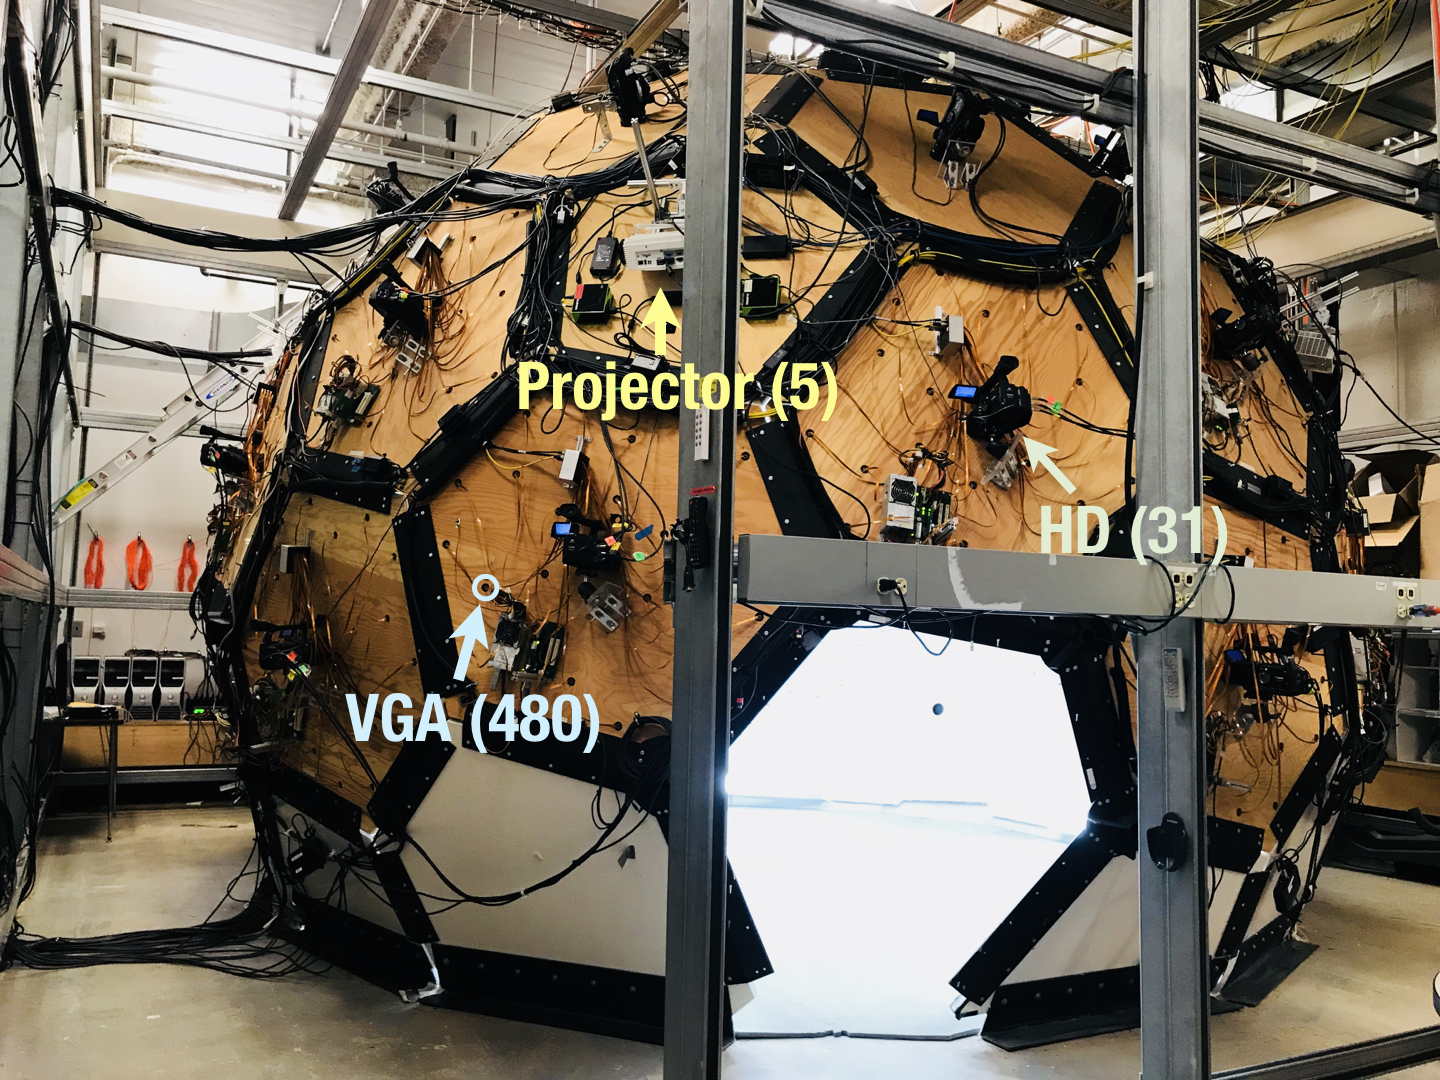
\includegraphics[trim=0 0 0 0,clip,width=\linewidth]{fig_system/dome_exterior2_label}
	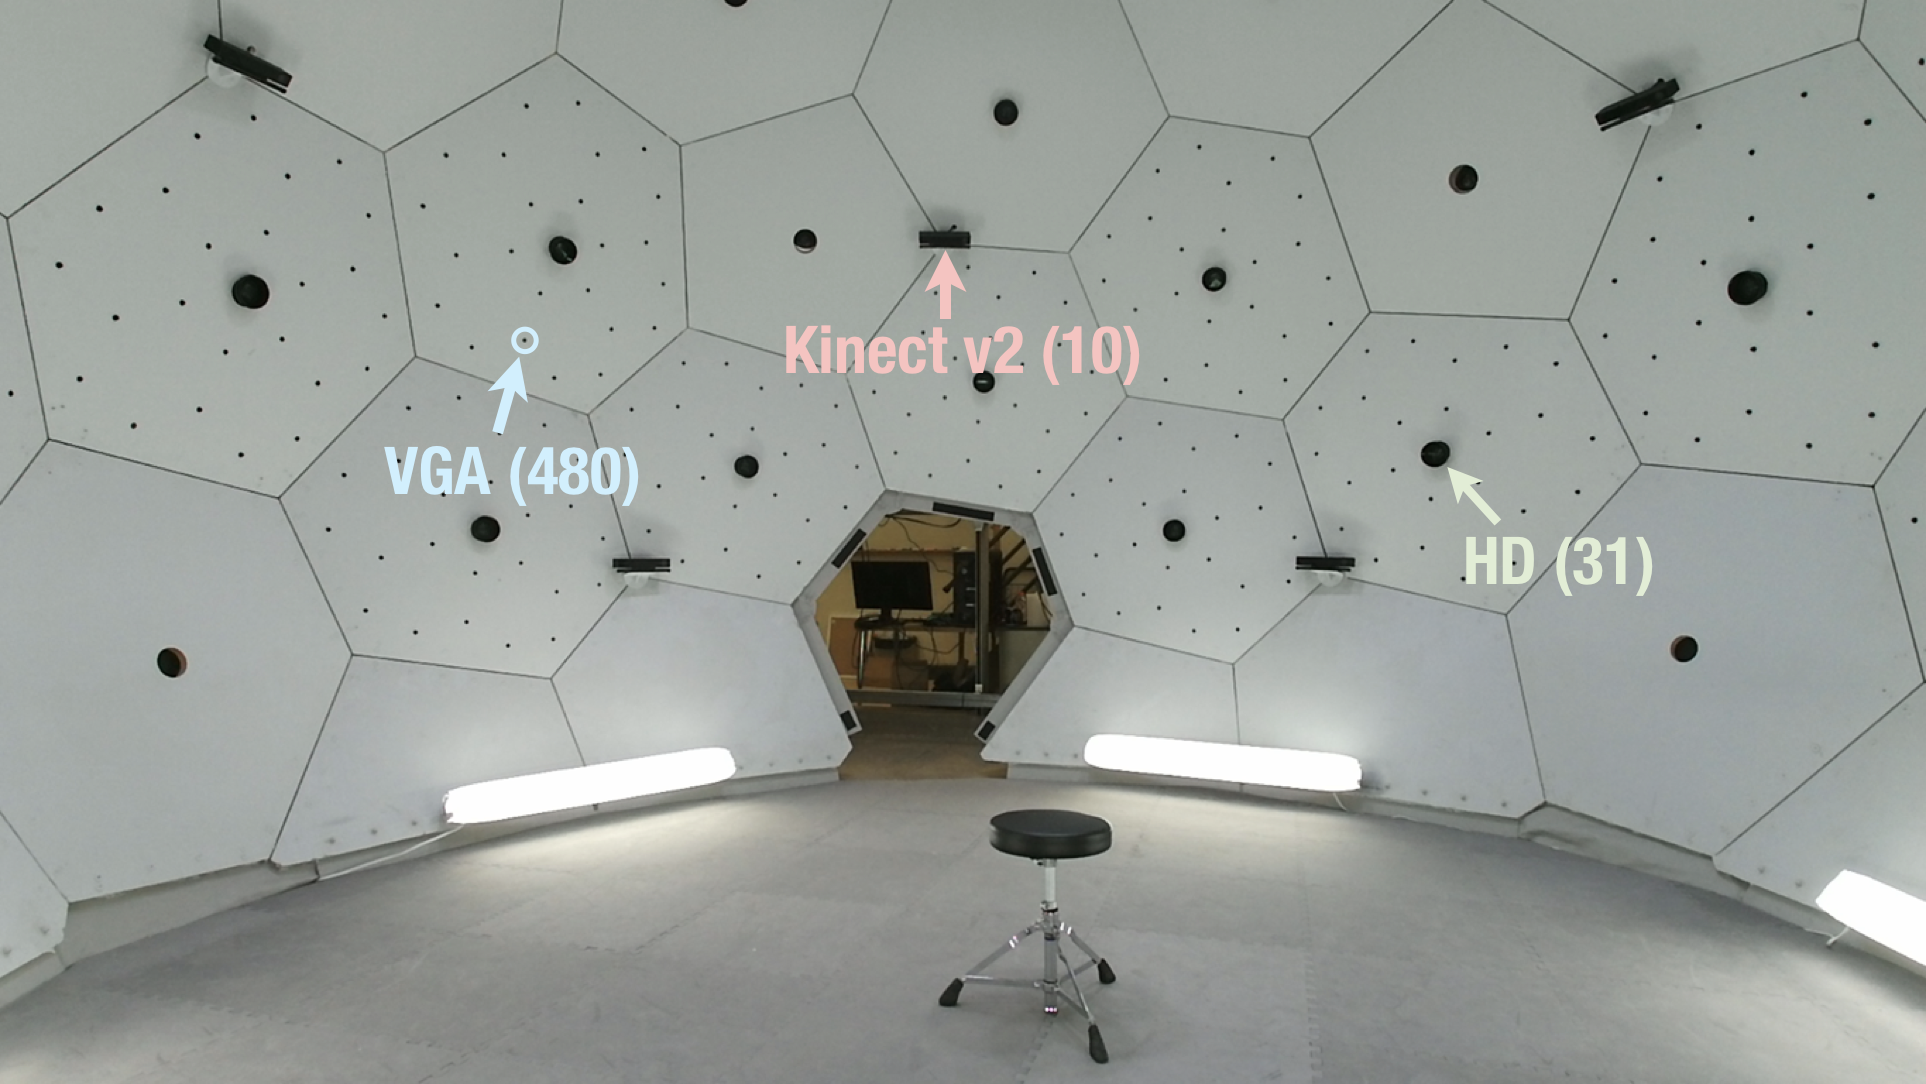
\includegraphics[trim=0 0 0 0,clip,width=\linewidth]{fig_system/panoptic_inside}	
	\caption{The exterior and interior shape of the Panoptic Studio, equipped with  480 VGA cameras, 31 HD cameras, 10 RGB+D cameras, and 5 DLP Projectors. (Top) The exterior of the Panoptic Studio. (Bottom) The interior of the Panoptic Studio.} 
	\label{fig:dome_ext_int}
\end{figure}

\begin{figure}
	\centering       
	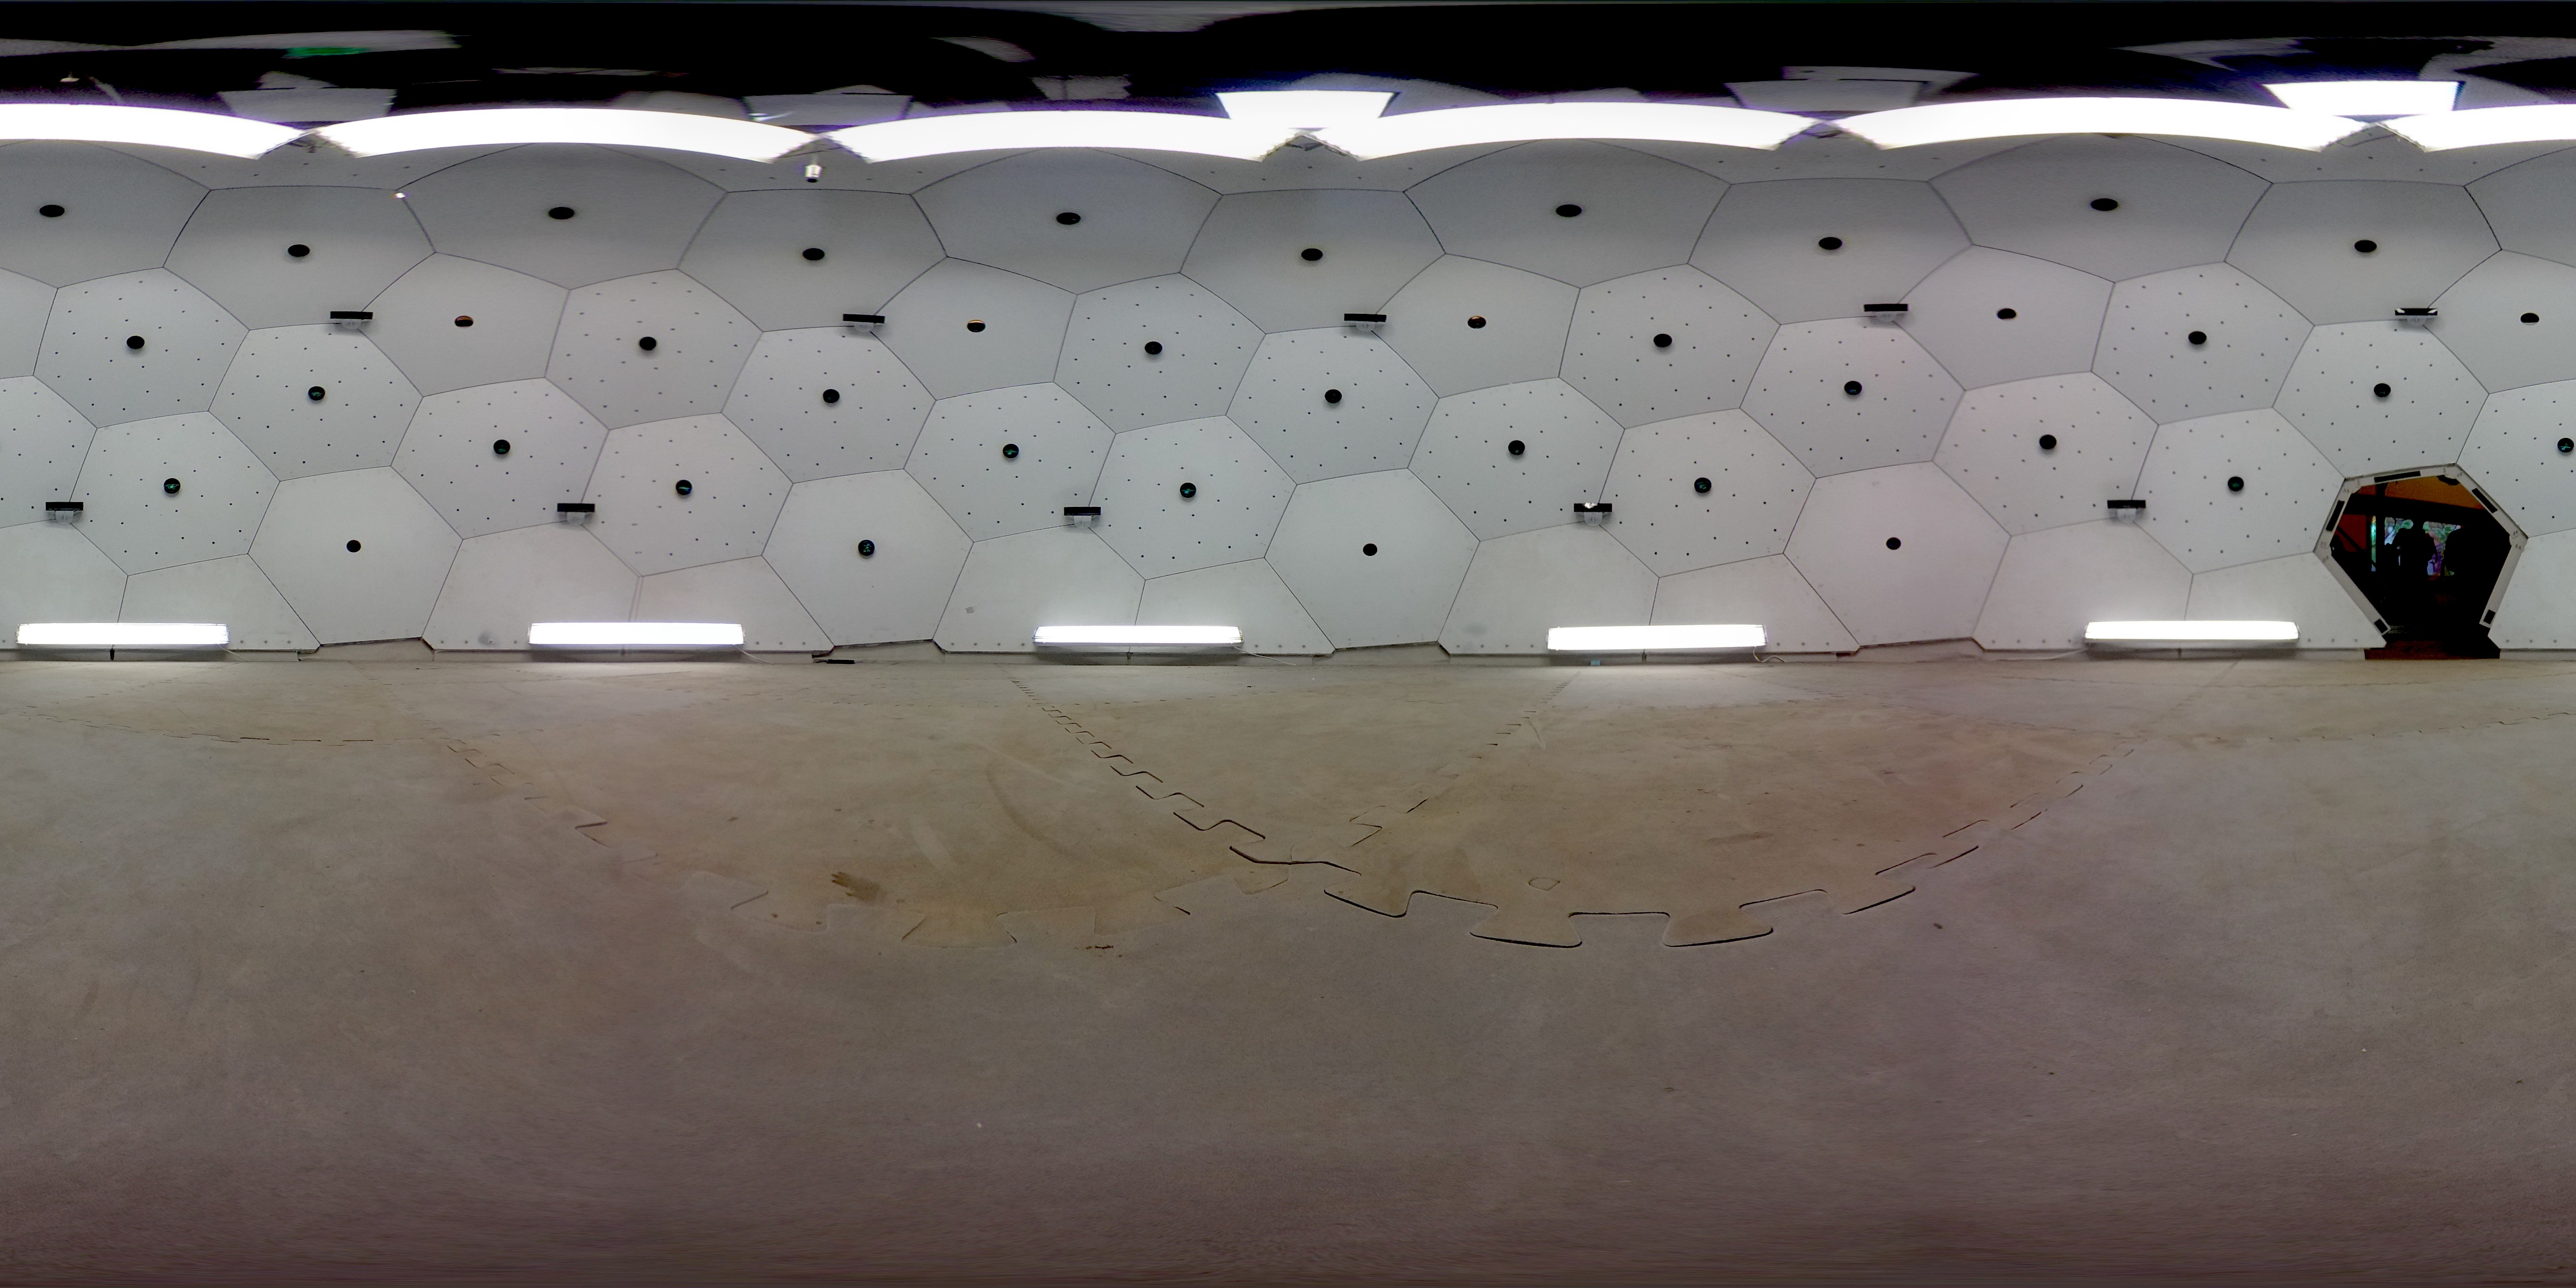
\includegraphics[trim=0 0 0 0,clip,width=\linewidth]{fig_system/dome_pano}	
	\caption{A 360\degree~panoramic photo captured inside the Panoptic Studio. The empty panel is the entrance of the studio.} 
	\label{fig:dome_panorama}
\end{figure}

\begin{figure}
	\centering       
	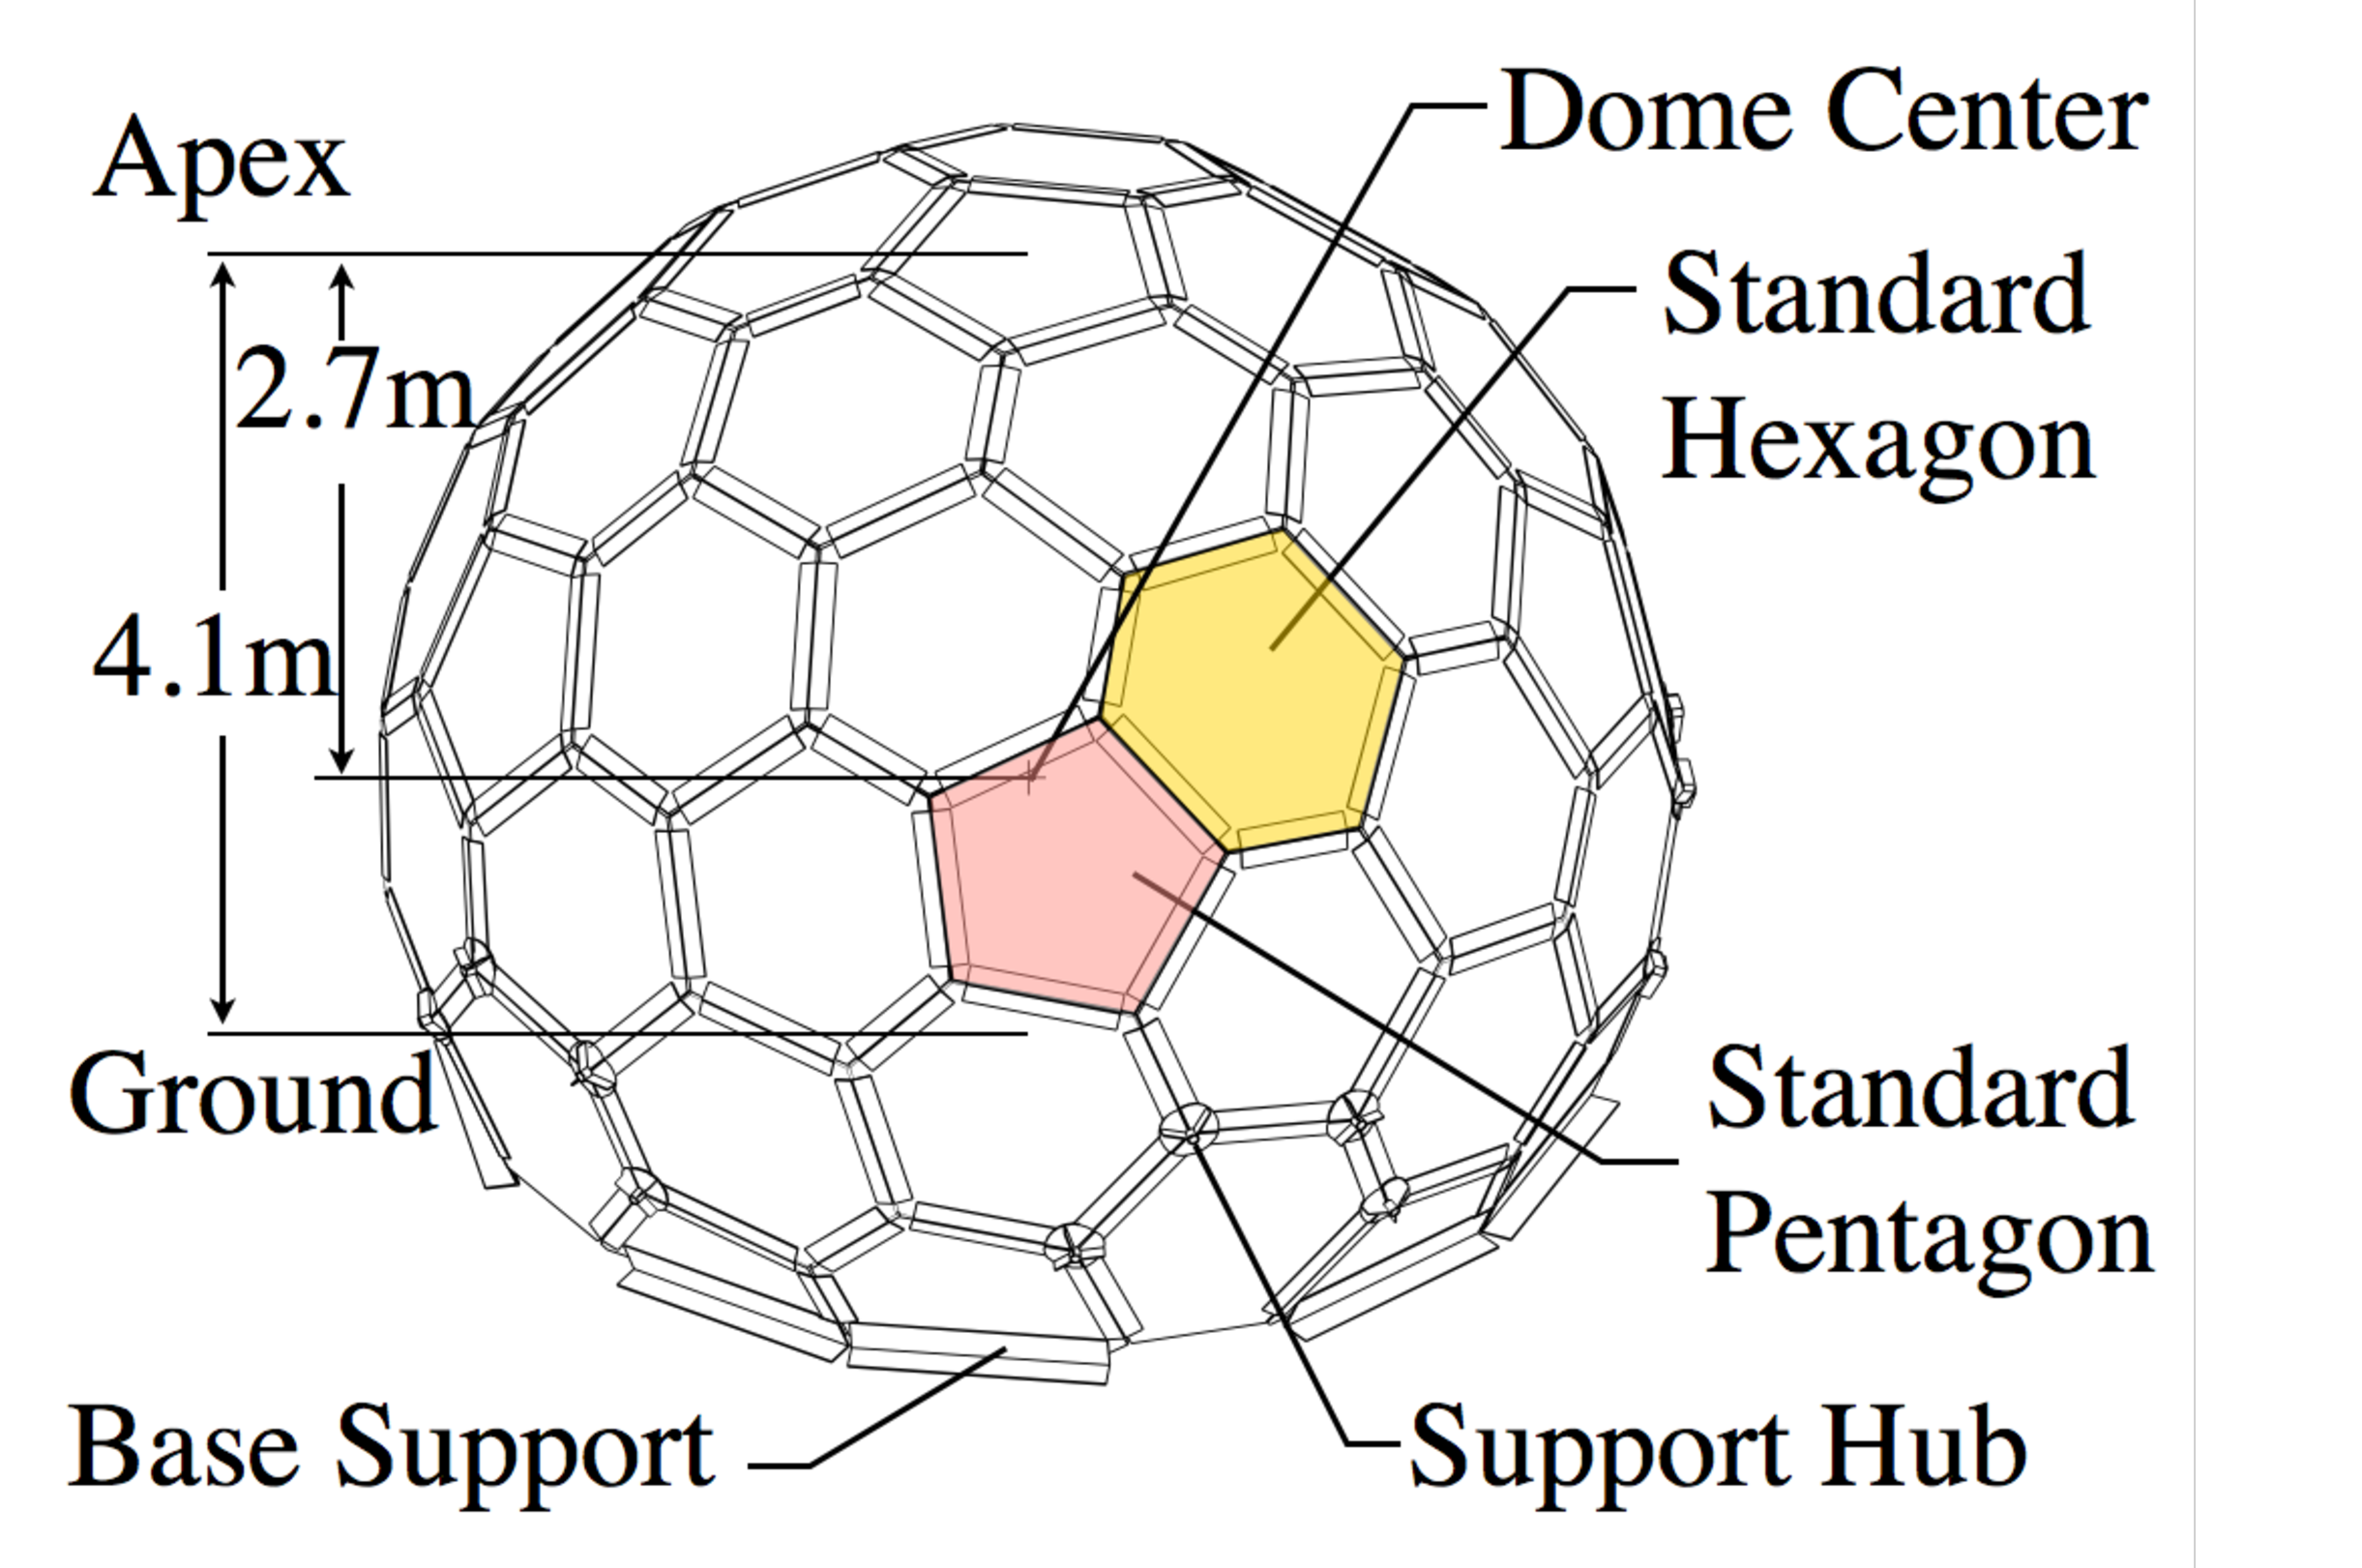
\includegraphics[trim=0 0 100 0,clip,width=0.48\linewidth]{figures/DomeFigure2} 
	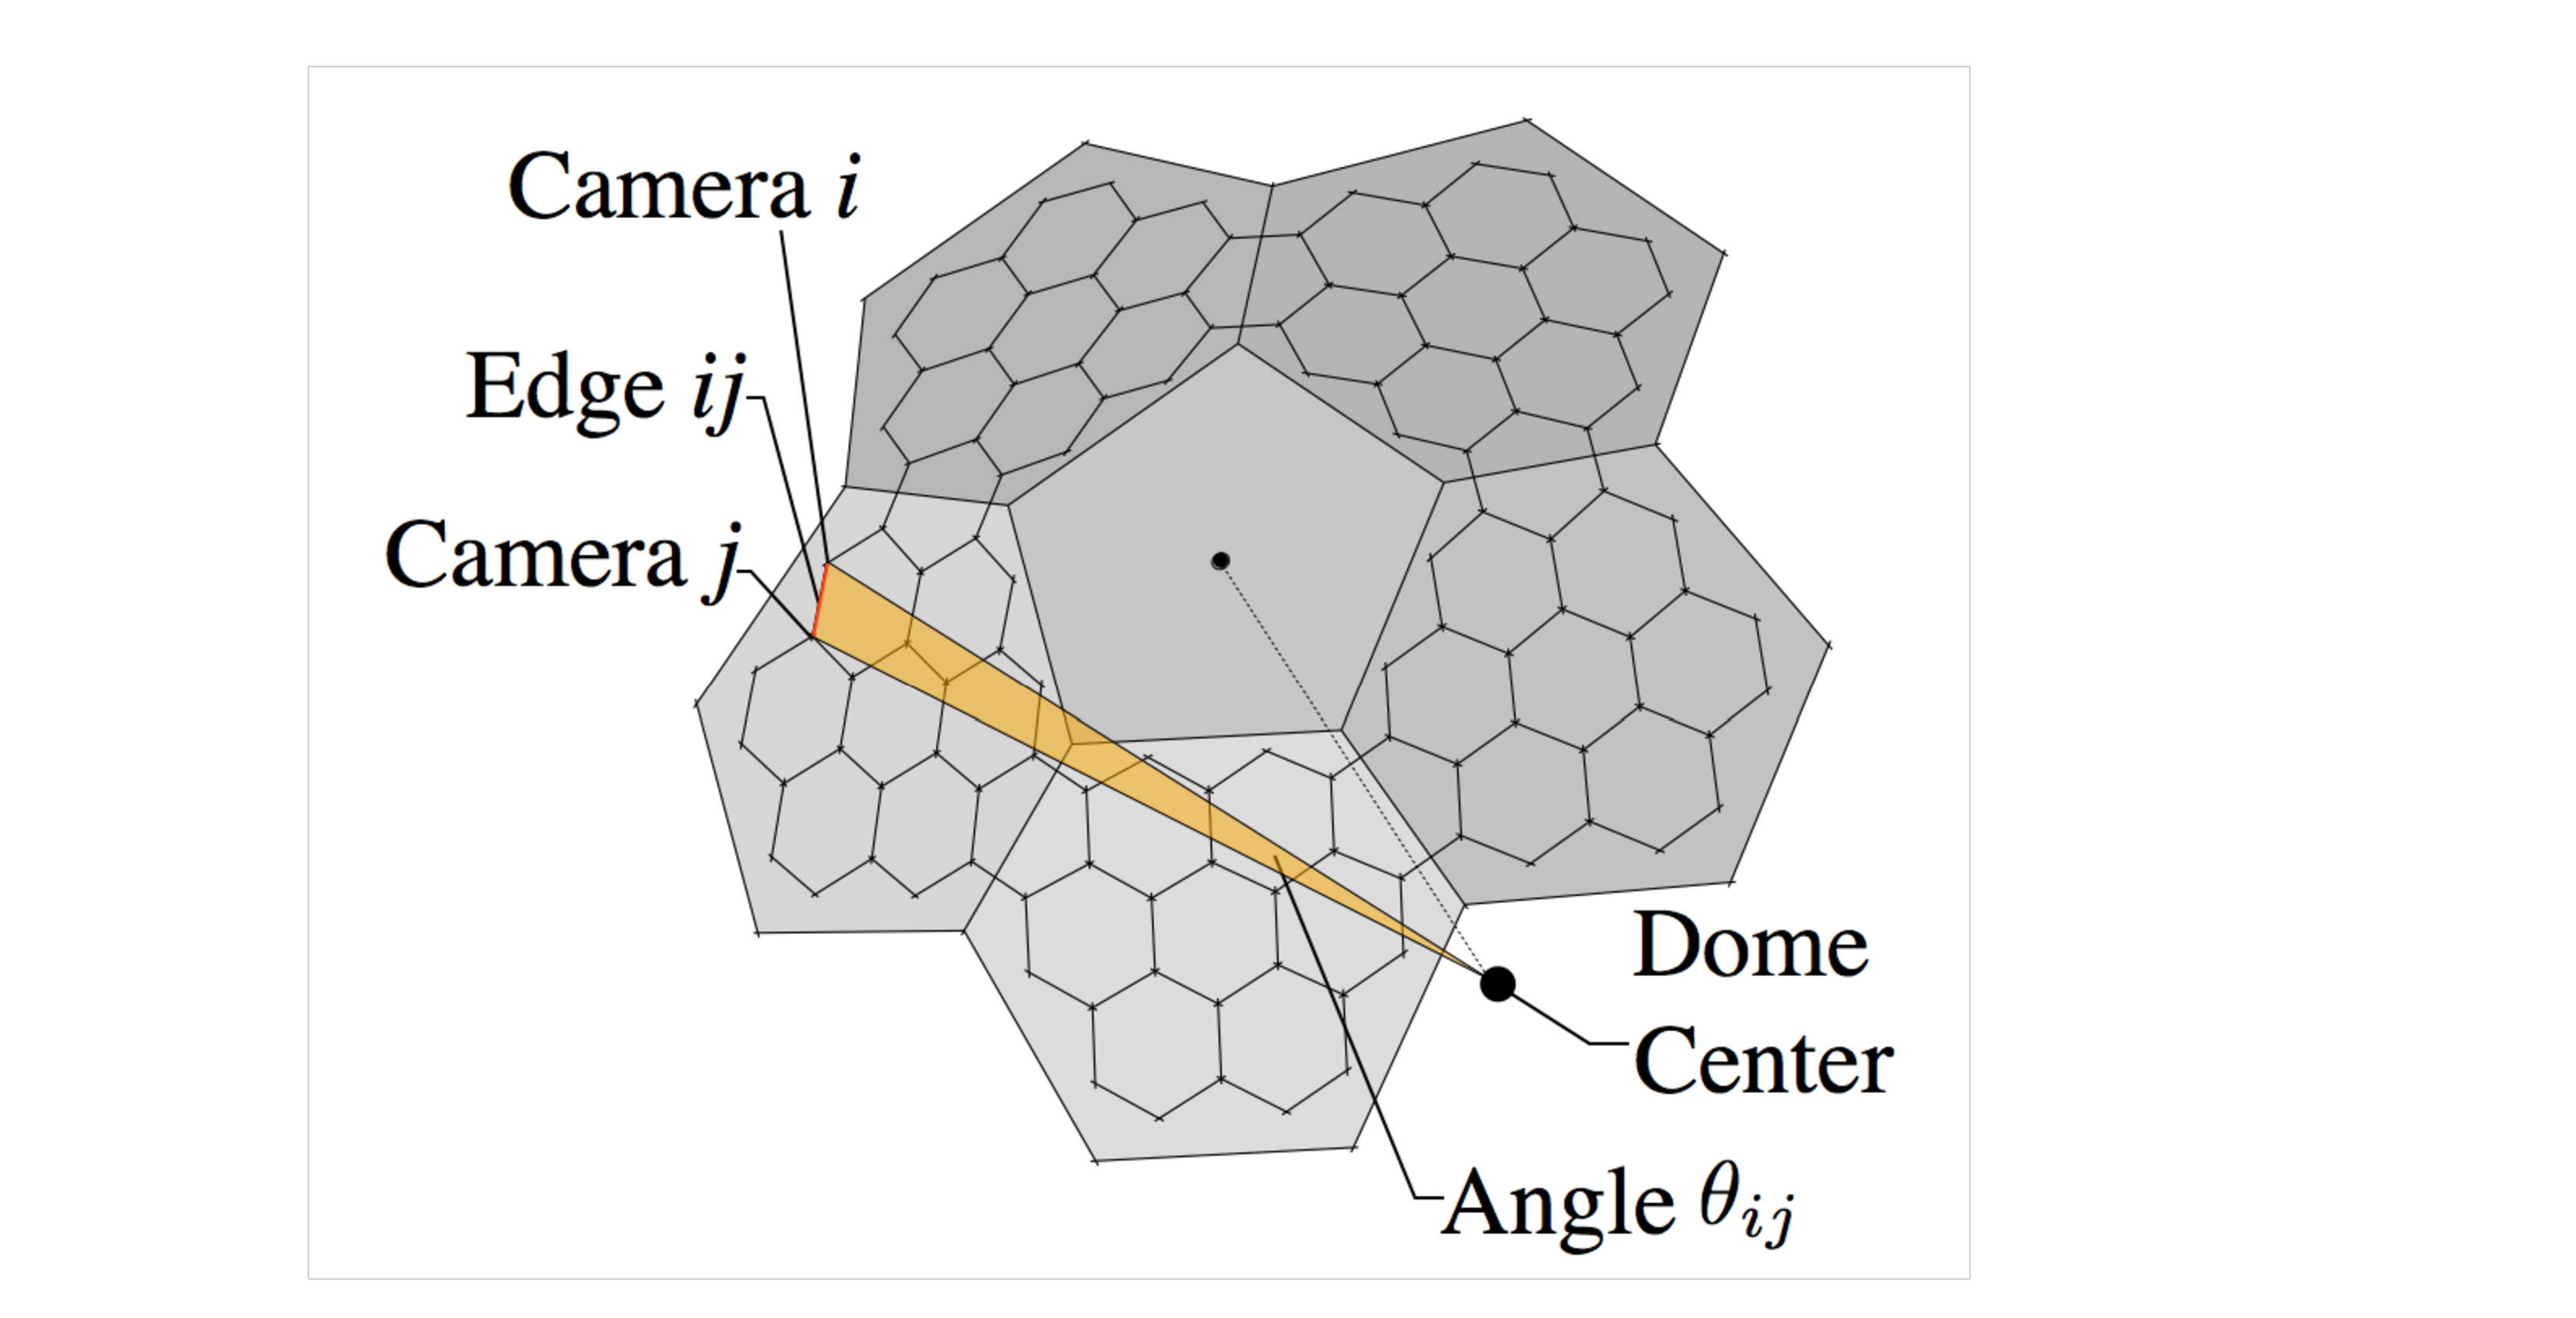
\includegraphics[trim=230 50 400 50,clip,width=0.48\linewidth]{figures/DomeFigure3}
	\caption{Structural Design of the Panoptic Studio (Left) The system has a modularized design with repeated pentagon and hexagon shapes, to ensure interchangeability (Right) Optimized VGA camera positions to ensure uniform angles with respect to the dome center between each camera and all its neighbors (e.g., Camera $i$ is a neighbor of Camera $j$).} 
	\label{fig:dome_structure}
\end{figure}


Our design was modularized so that each hexagonal panel houses a set of 24 VGA cameras and a HD camera. To determine the placement of the VGA cameras, we initialized their positions by tessellating the hexagon face into 24 triangles and using this initialization to define a 3-neighborhood structure shown in the right of Figure~\ref{fig:dome_structure}. Using this neighborhood structure and the initialization we determine the placement of the cameras over the geodesic dome by minimizing the difference in angles between all neighbors of every camera,

{\small
	\begin{equation}\nonumber
	\{\theta_{ij}\}^* = \arg \min_{\{\theta_{ij}\}} \sum_{p=1}^P \sum_{i=1}^{N} \sum_{j \in \mathcal{N}(i)}  \sum_{k \in \mathcal{N}(i) \neq j}  (r(\theta_{ij}|p)-r(\theta_{ik}|p))^2 ,
	\end{equation}
}where $P=20$ is the number of panels, $N=24$ is the number of cameras in each panel, $\mathcal{N}(\cdot)$ is the neighborhood of a camera, $r(\cdot|p)$ is a function transforming the angle on a reference panel to the $p$-th panel. The cameras sample the span of the vertical axis of the space and sample $48.71^\circ$ of the horizontal axis. With this distribution, the minimum baseline between any VGA camera and its nearest three neighbors is 21.05cm. 
	
The 31 HD cameras are installed at the center of each hexagonal panel, and 5 projectors are installed at the center of each pentagonal panel\footnote{Note that no sensors are installed on some panels (e.g., ceiling panels occluded by lights).}. Additionally, a total of 10 Kinect v2 RGB+D sensors are mounted at heights of 1 and 2.6 meters, forming two rings with 5 evenly spaced sensors each. %The interior and exterior of our system are shown in Figure~\ref{fig:domeFigure}, and components of our system is shown in Figure~\ref{fig:domeEquipment}


		 %Naturally, there is some variation in this number due to the physical imprecision of mounting.
	%Placement of cameras.
	%Williams, Robert (1979). The Geometrical Foundation of Natural Structure: A Source Book of Design. Dover Publications, Inc. ISBN 0-486-23729-X. (Section 3-9)
	% \noindent \textbf{Acquisition Hardware.} The dome has twenty panels, each with 24 VGA cameras and one HD camera, for a total for 480 VGA cameras and 16 HD cameras. The sensors are arranged to lie uniformly around the twenty panels. 
	
%	\begin{figure}
%	\centering       
%	%	\subfigure{\label{fig:domeFigure1}\includegraphics[trim=400 0 150 0,clip,width=0.45\linewidth]{imgs/Dome_outside}} 
%	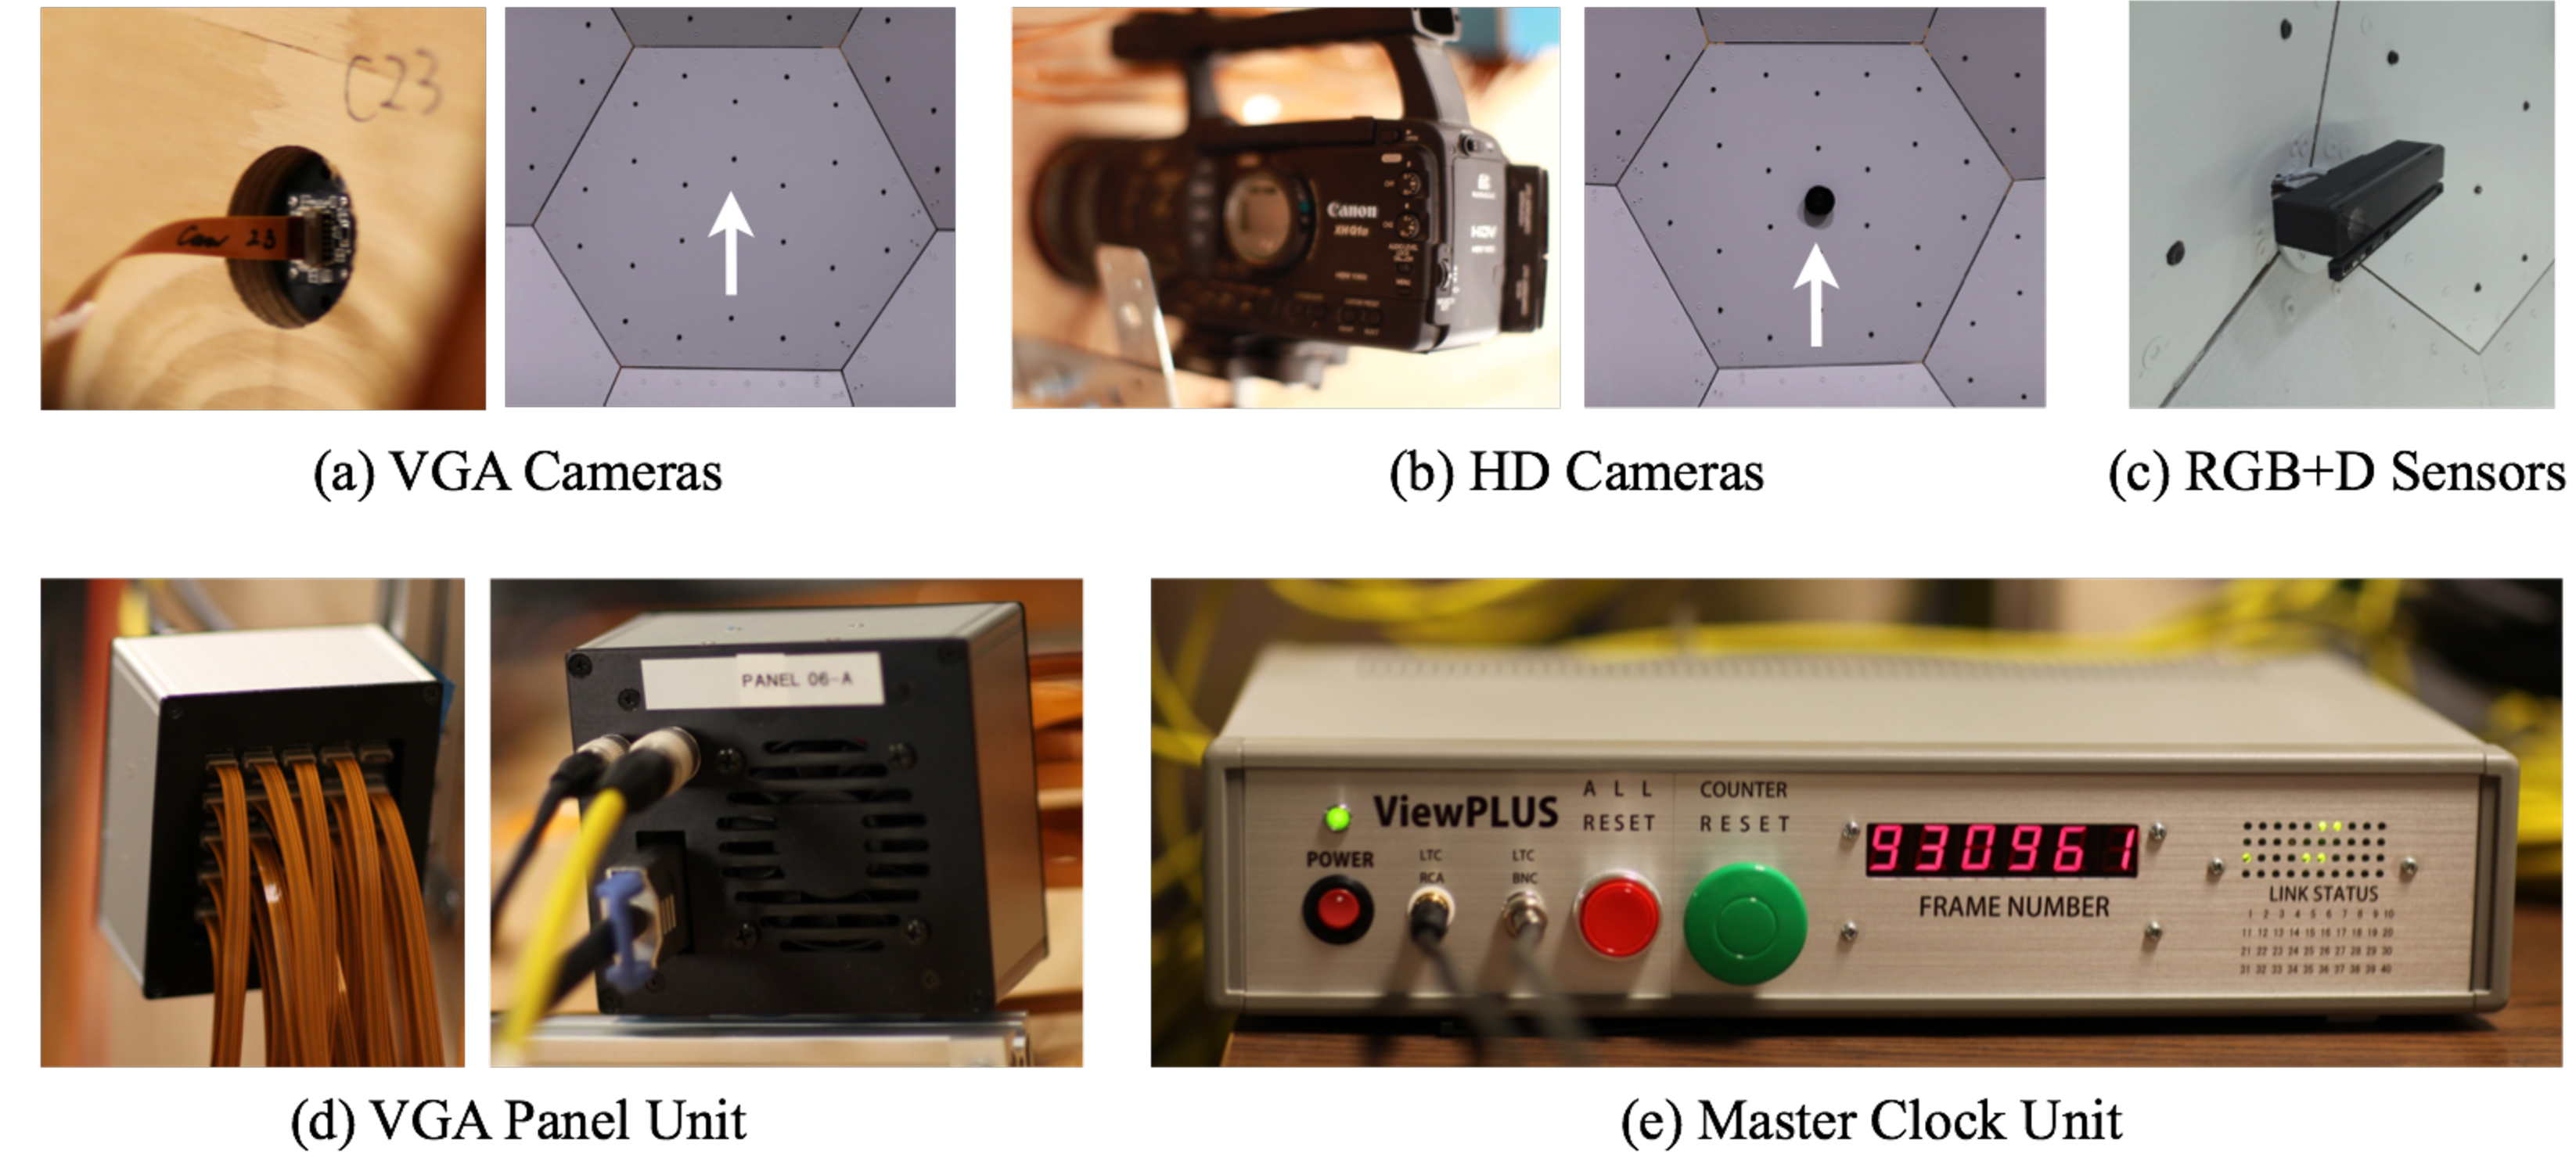
\includegraphics[trim=0 0 0 0,clip,width=\linewidth]{figures/Equipment}
%	\caption{Sensors and equipments installed in the Panoptic Studio. } 
%	\label{fig:domeEquipment}
%\end{figure}
\section{System Architecture}
%which consists of 480 VGA cameras, 31 HD cameras, 10 Kinect v2 RGB+D sensors, and 5 DLP projectors. 
Figure \ref{fig:dome_architecture} shows the architecture of our system. The panoptic studio is composed of four sub-systems: VGA camera system, HD camera system, RGB-D camera system, and projector system.
\mbox{ }\\
\noindent \textbf{VGA Camera System:} The 480 cameras are arranged modularly with 24 cameras in each of 20 standard hexagonal panels on the dome. Each module in each panel is managed by a Distributed Module Controller (DMC) that triggers all cameras in the module, consolidates the videos from cameras, and transmits the data to the local machine. Each individual camera has a global shutter CMOS sensor, with a fixed focal length of 4.5mm, capturing VGA ($640\times480$) resolution images at 25Hz. The detailed configuration is shown in Figure~\ref{fig:dome_vgaSystem}. 

\begin{figure}[t]
	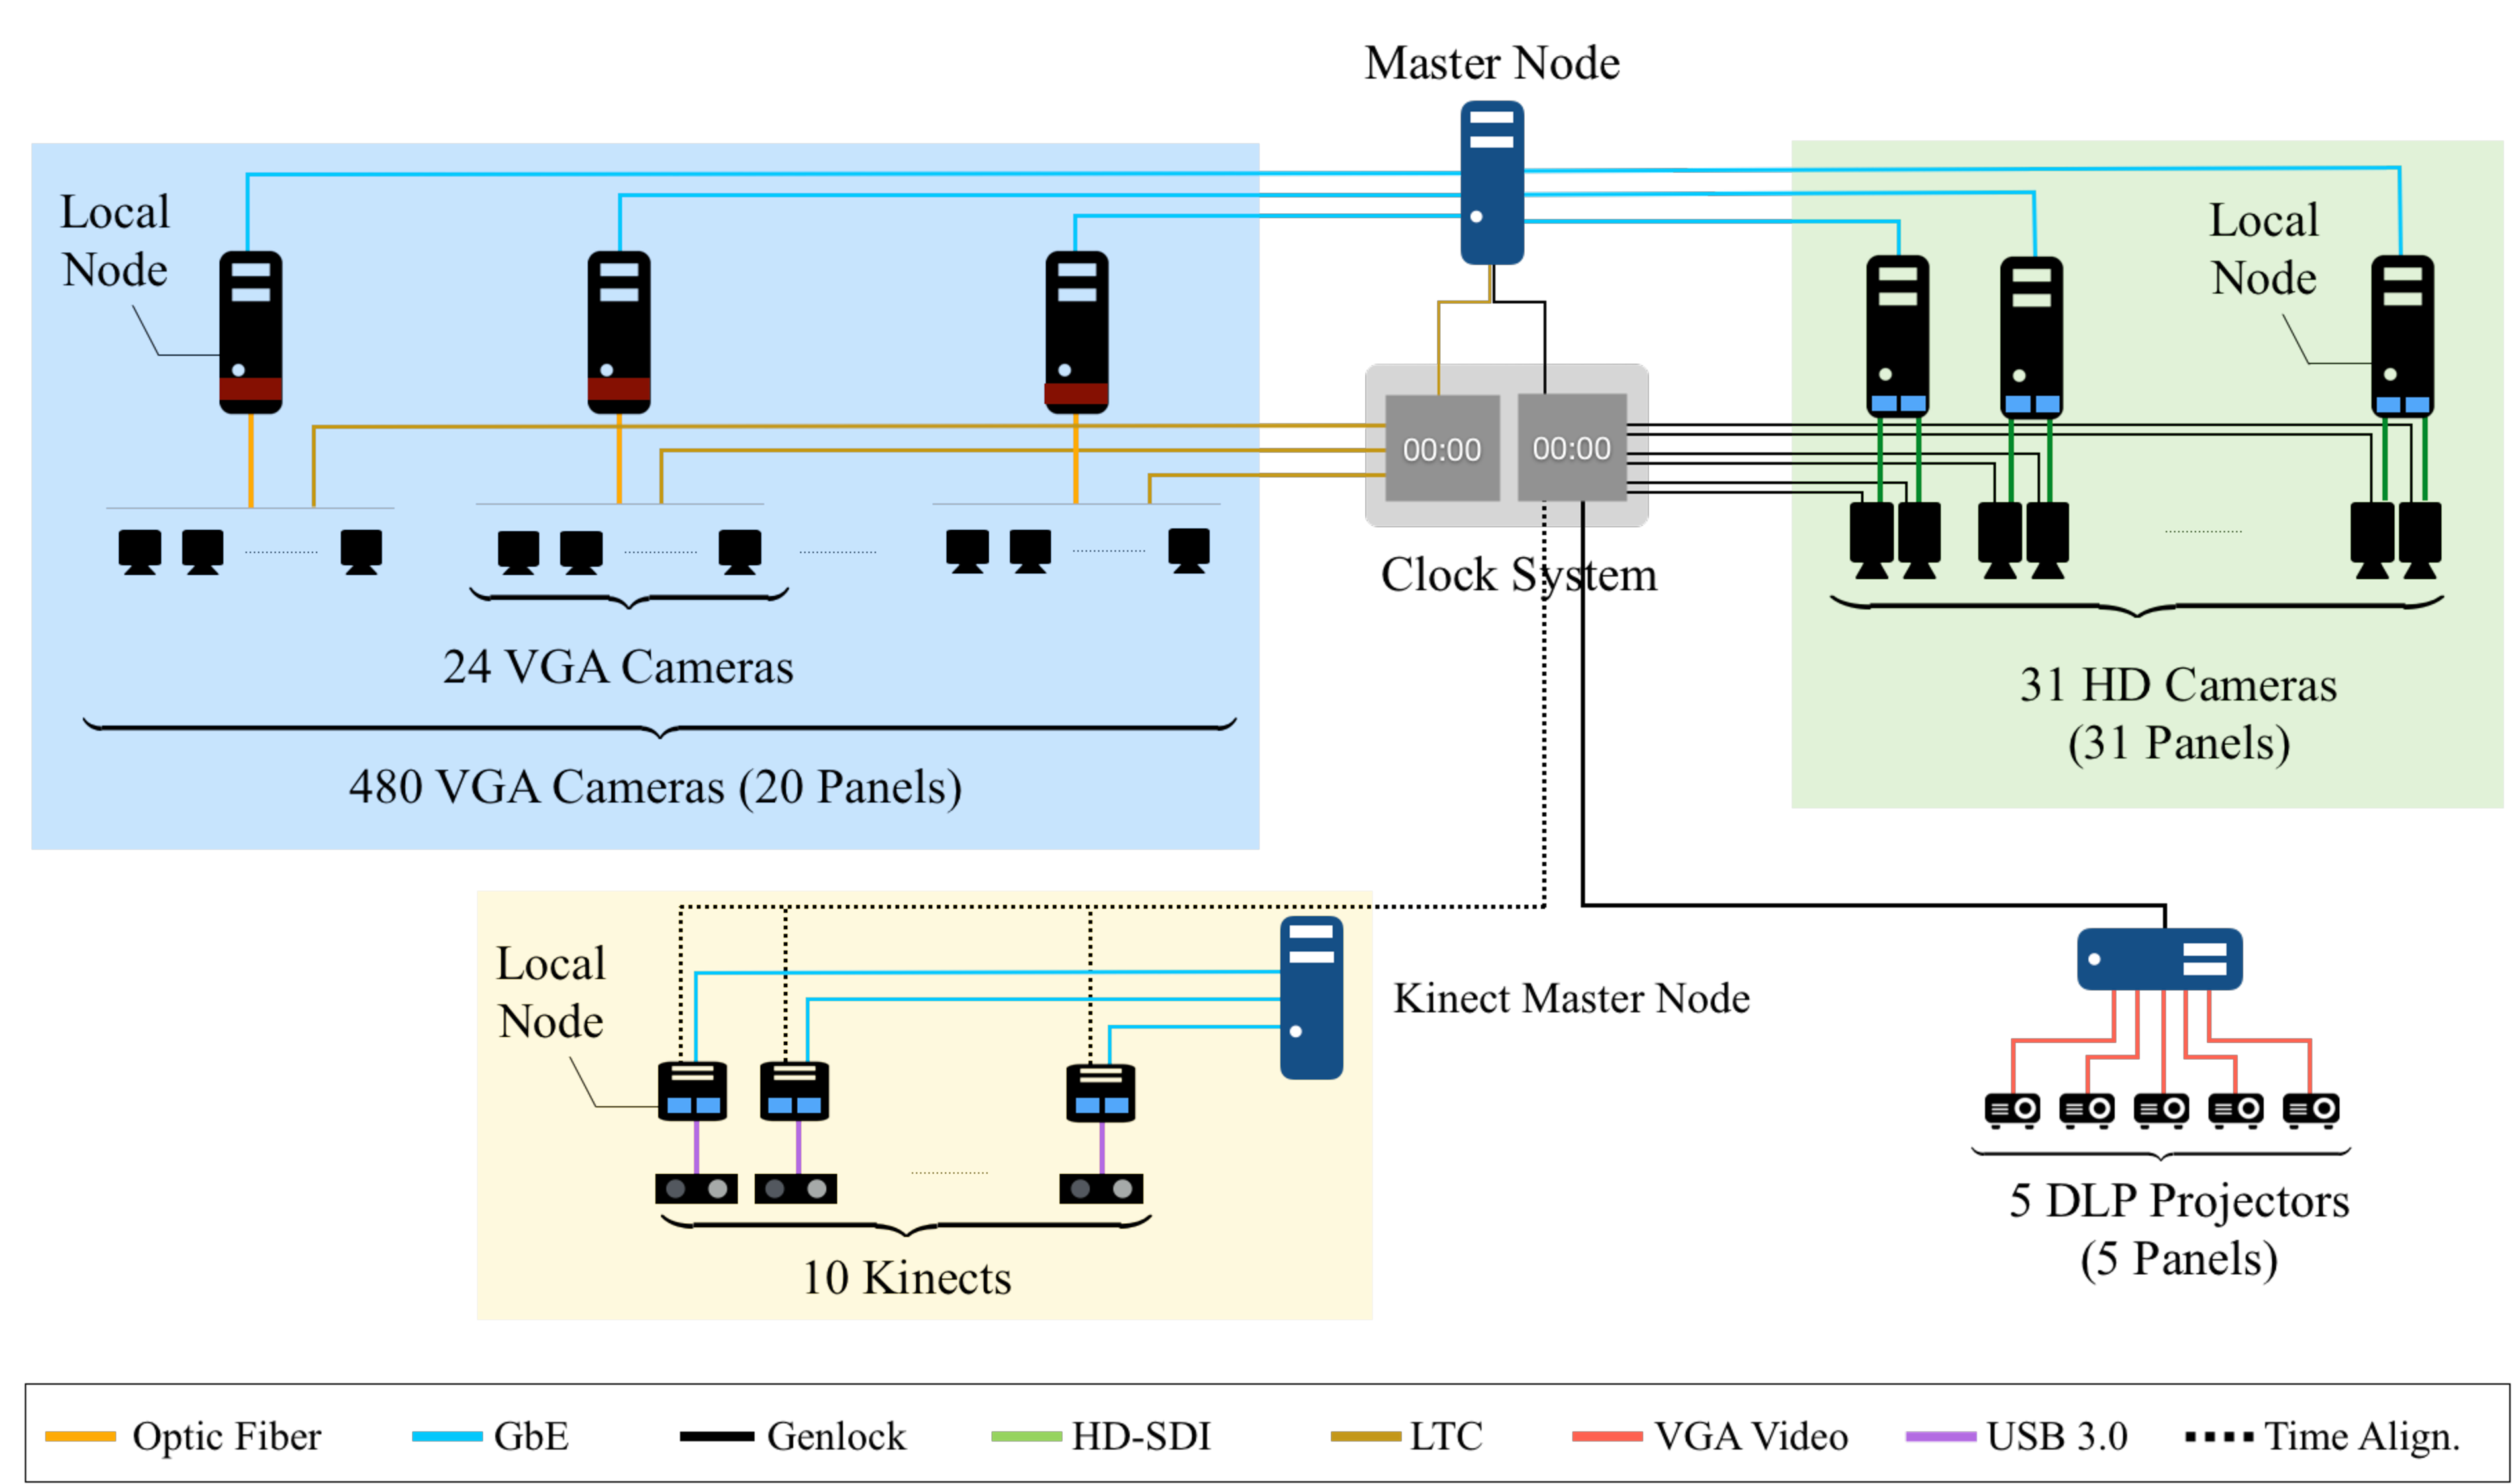
\includegraphics[width=\linewidth]{fig_system/panoptic_architecture}
	%\includegraphics[width=\linewidth]{images/Design6.pdf}
	%	\vspace{-0.2in}
	\caption{Modularized system architecture. The system is composed of four sub-systems, depending on sensor types. The studio houses 480 VGA cameras, 31 HD cameras, 10 RGB+D sensors, and 5 DLP projectors. The 480 VGA cameras are synchronized by a clock system with 25 Hz, and HD cameras and projectors are synchronized by another clock system with 29.97 Hz. Both clocks are temporally aligned by recording them as a stereo signal. 10 RGB-D sensors are also time-aligned in the common time domain. All the sensors are spatially calibrated to the same coordinate system.}
	\label{fig:dome_architecture}
\end{figure}

Each panel produces an uncompressed video stream at 1.47 Gbps, and thus, the data-rate of the entire set of 480 cameras is approximately 29.4 Gbps. To handle this stream, the system pipeline has been designed with a modularized communication and control structure. For each module, the clock generator sends a frame counter, trigger signal, and the pixel clock signal to each DMC associated with a panel. The DMC uses this timing information to initiate and synchronize capture of all cameras within the module. Upon trigger and exposure, each of the 24 camera heads transfers back image data via the camera interconnect to the DMC, which consolidates the image data and timing from all cameras. This composite data is then transferred via optical interconnect to the module node, where it is stored locally. The 20 local nodes for VGA camera system are shown in the left of the Figure~\ref{fig:dome_machines}. Each local node for a module has dual purpose: it serves as a distributed RAID storage unit\footnote{Each node has 3 HDDs integrated as RAID-0 to have sufficient write speed without data loss, totaling 60 HDDs for 20 modules.} and participates as a multi-core computational node in a cluster. All the local nodes of our system are on a local network on a gigabit switch. The acquisition is controlled via a master node that a system operator can use to control all functions of the studio.


\begin{figure}
	\centering       
	\includegraphics[trim=0 0 0 0,clip,width=\linewidth]{fig_system/vga_system}	
	\caption{A VGA camera module. We use a customized camera array with 24 VGA cameras as a single module. Each module is controlled by a camera controller that is connected to a small desktop machine. They are attached to the panel. The small desktop machine is connected to a single VGA node machine, to transfer captured data.} 
	\label{fig:dome_vgaSystem}
\end{figure}


\begin{figure}
	\centering       
	\includegraphics[trim=0 0 0 0,clip,width=\linewidth]{fig_system/hd_system}	
	\caption
	{An HD camera module. We use an off-the-shelf HD camcorder with external genlock and timecode signals for the synchronization. Two HD cameras are connected to a single HD machine.} 
	\label{fig:dome_hdSystem}
\end{figure}

\begin{figure}[t]
	\centering       
	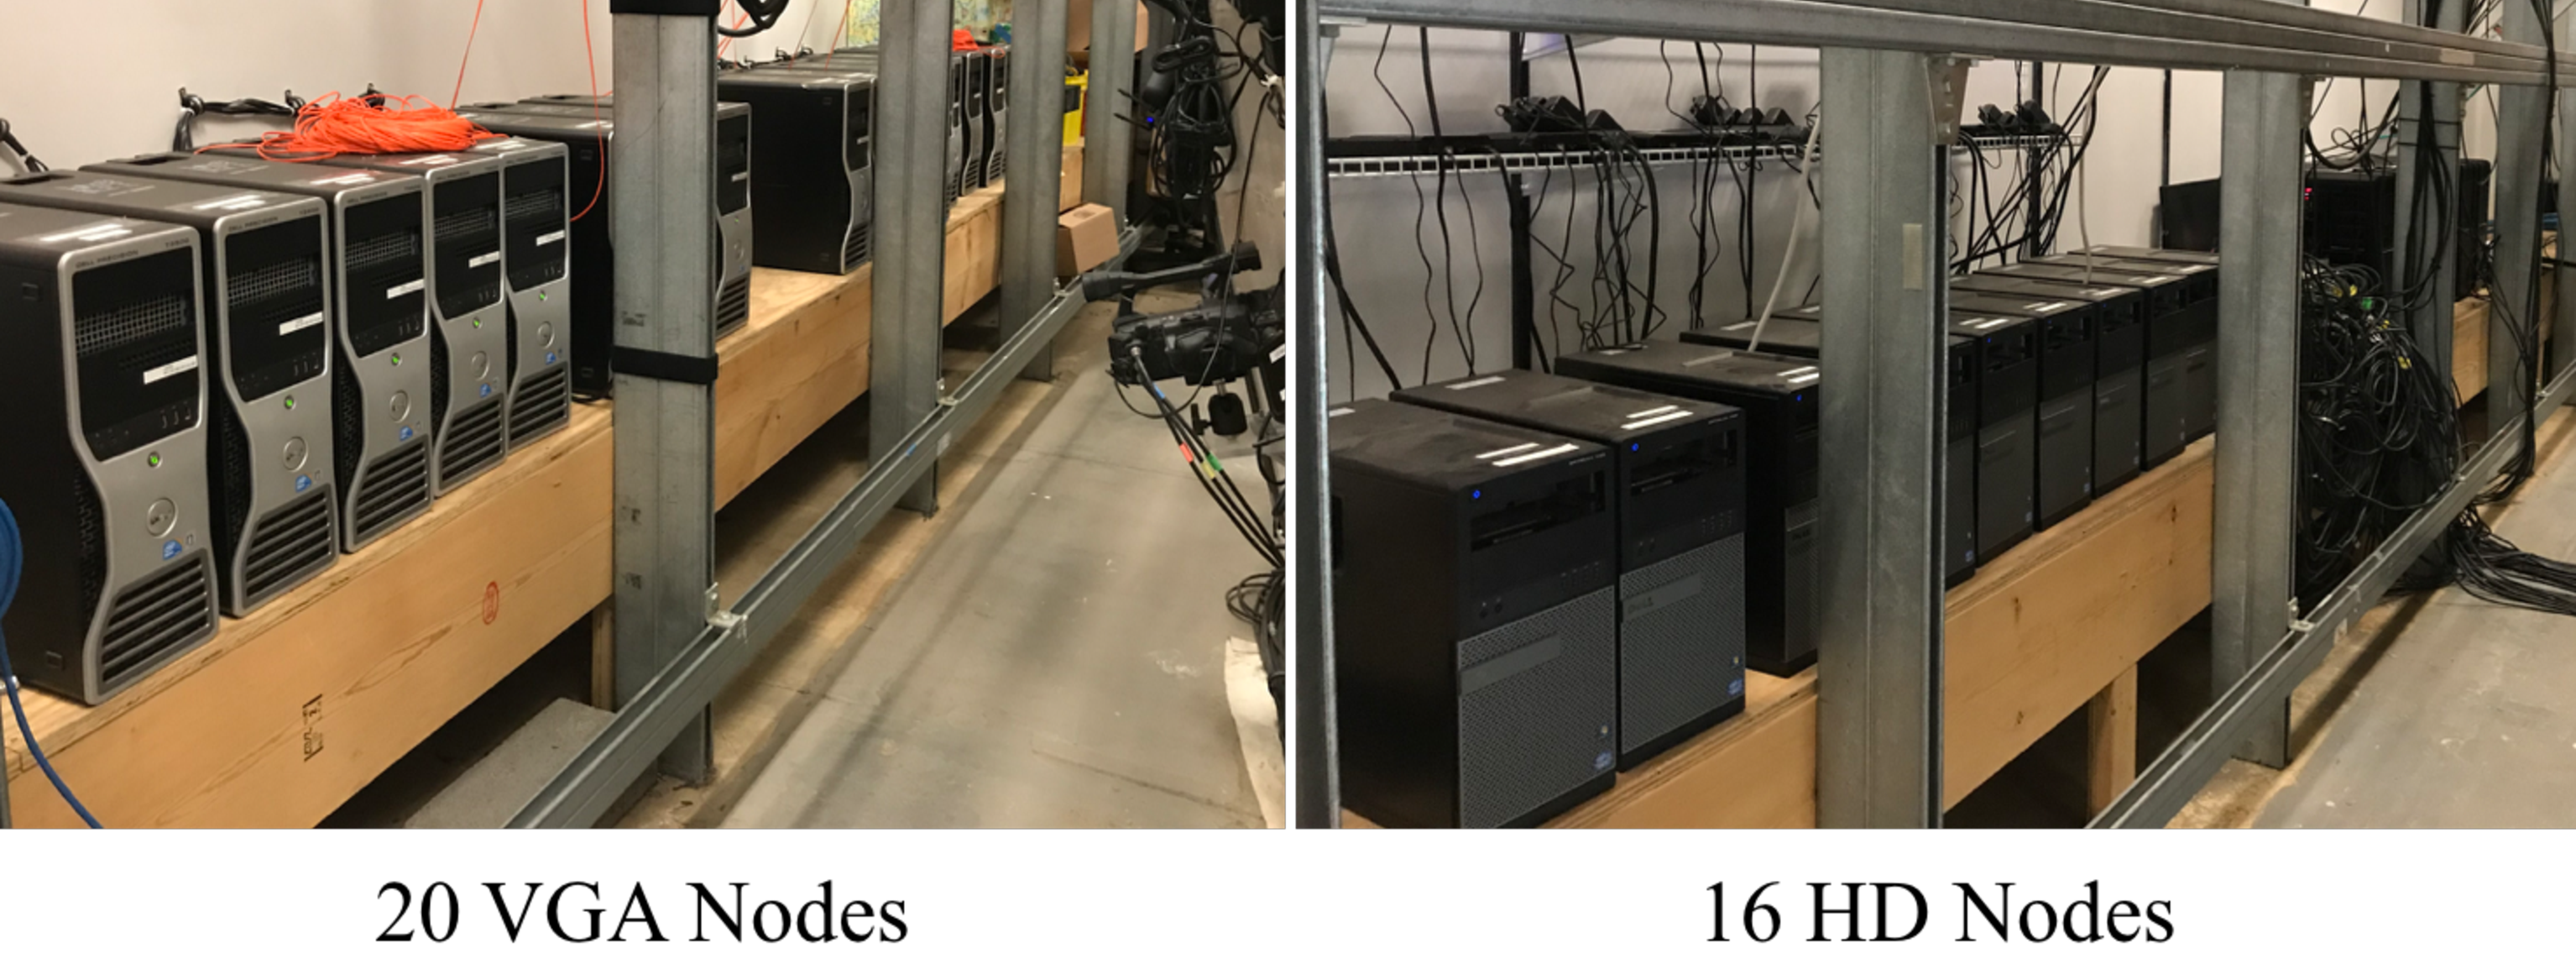
\includegraphics[trim=0 0 0 0,clip,width=\linewidth]{fig_system/machines}
	\caption{VGA subsystem is controlled by 20 node machines, and HD subsystem is controlled by 16 node machines. All nodes are connected and controlled by a master node to initiate the capture.}
	\label{fig:dome_machines}
\end{figure}
\begin{figure}[t]	
	\centering
	\begin{subfigure}{0.71\textwidth}
		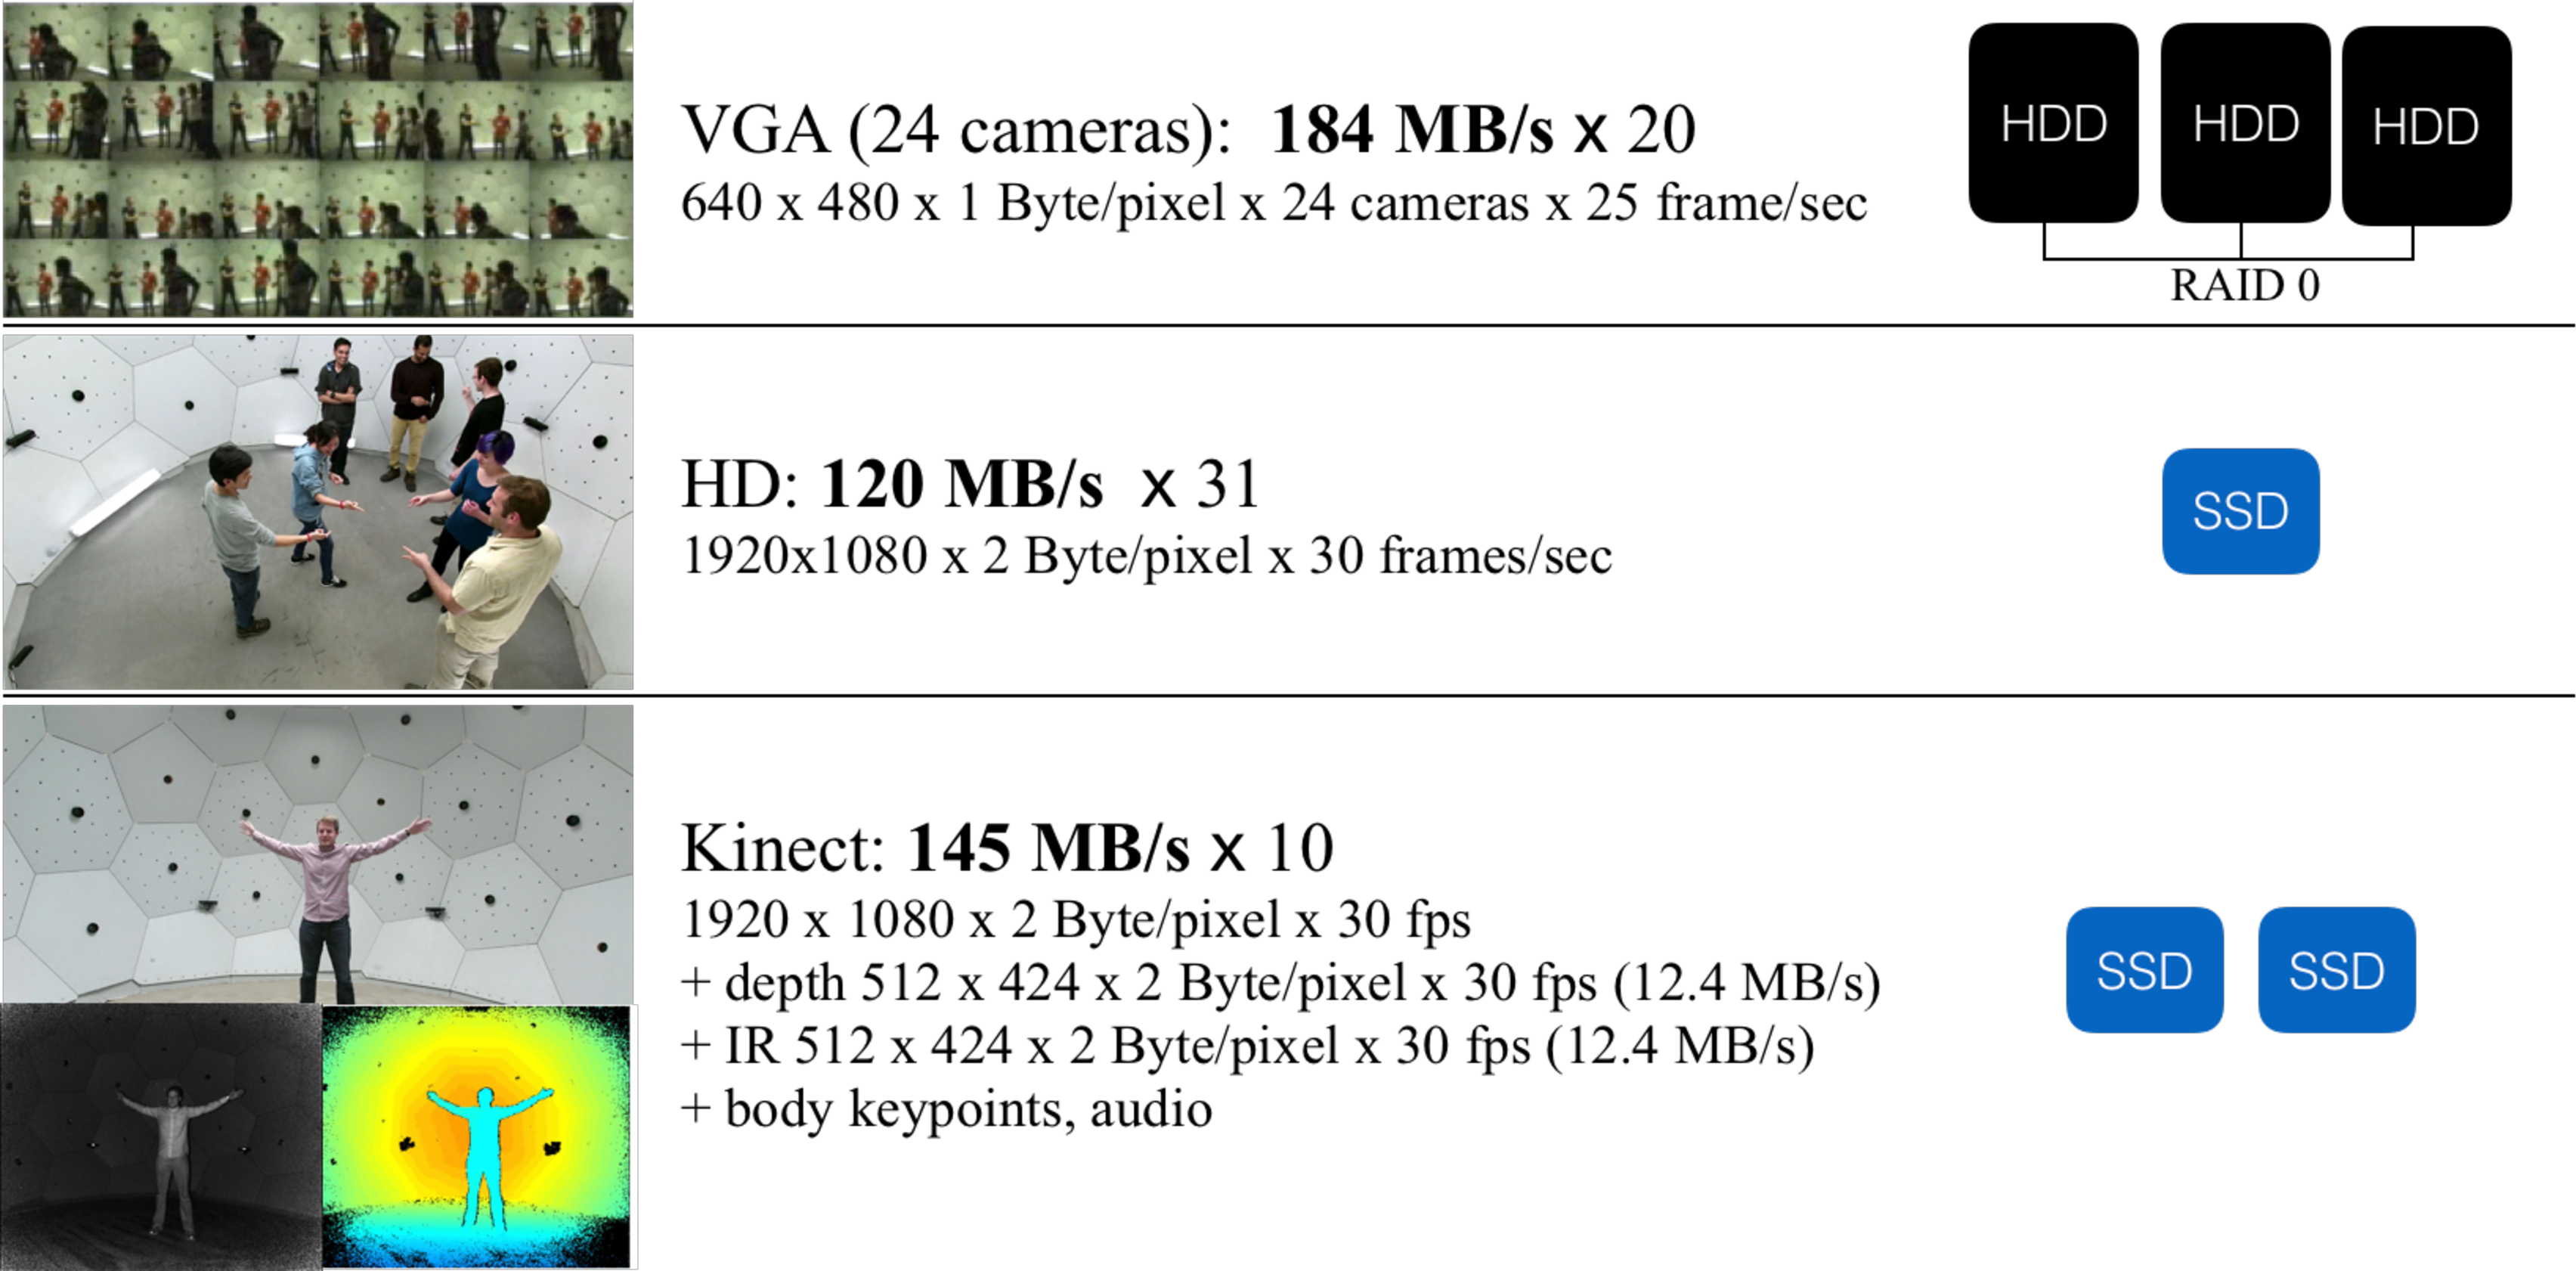
\includegraphics[width=\textwidth]{fig_system/storage}
		\caption{Data size and local storage for each node}
		\label{fig:dome_datasize}
	\end{subfigure}
	\begin{subfigure}{0.27\textwidth}
		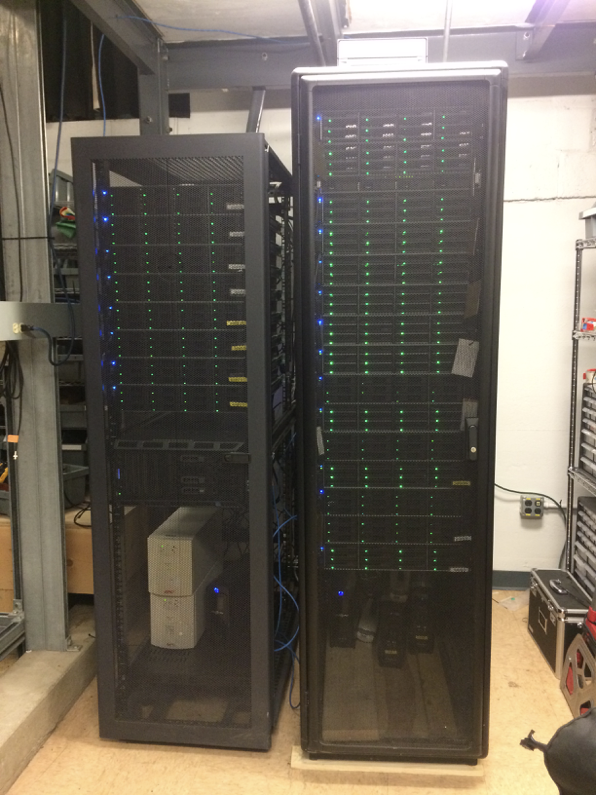
\includegraphics[width=\textwidth]{fig_system/dome_NAS}
		\caption{NAS sotrage system}
		\label{fig:dome_NAS}
	\end{subfigure}
	\caption{(a) Overall data size the Panoptic Studio generates per each second, and storage solutions for local nodes (b) Network Attached Storage (NAS) system to store the data for long-term.}
\end{figure}

\begin{figure}
	\centering       
	%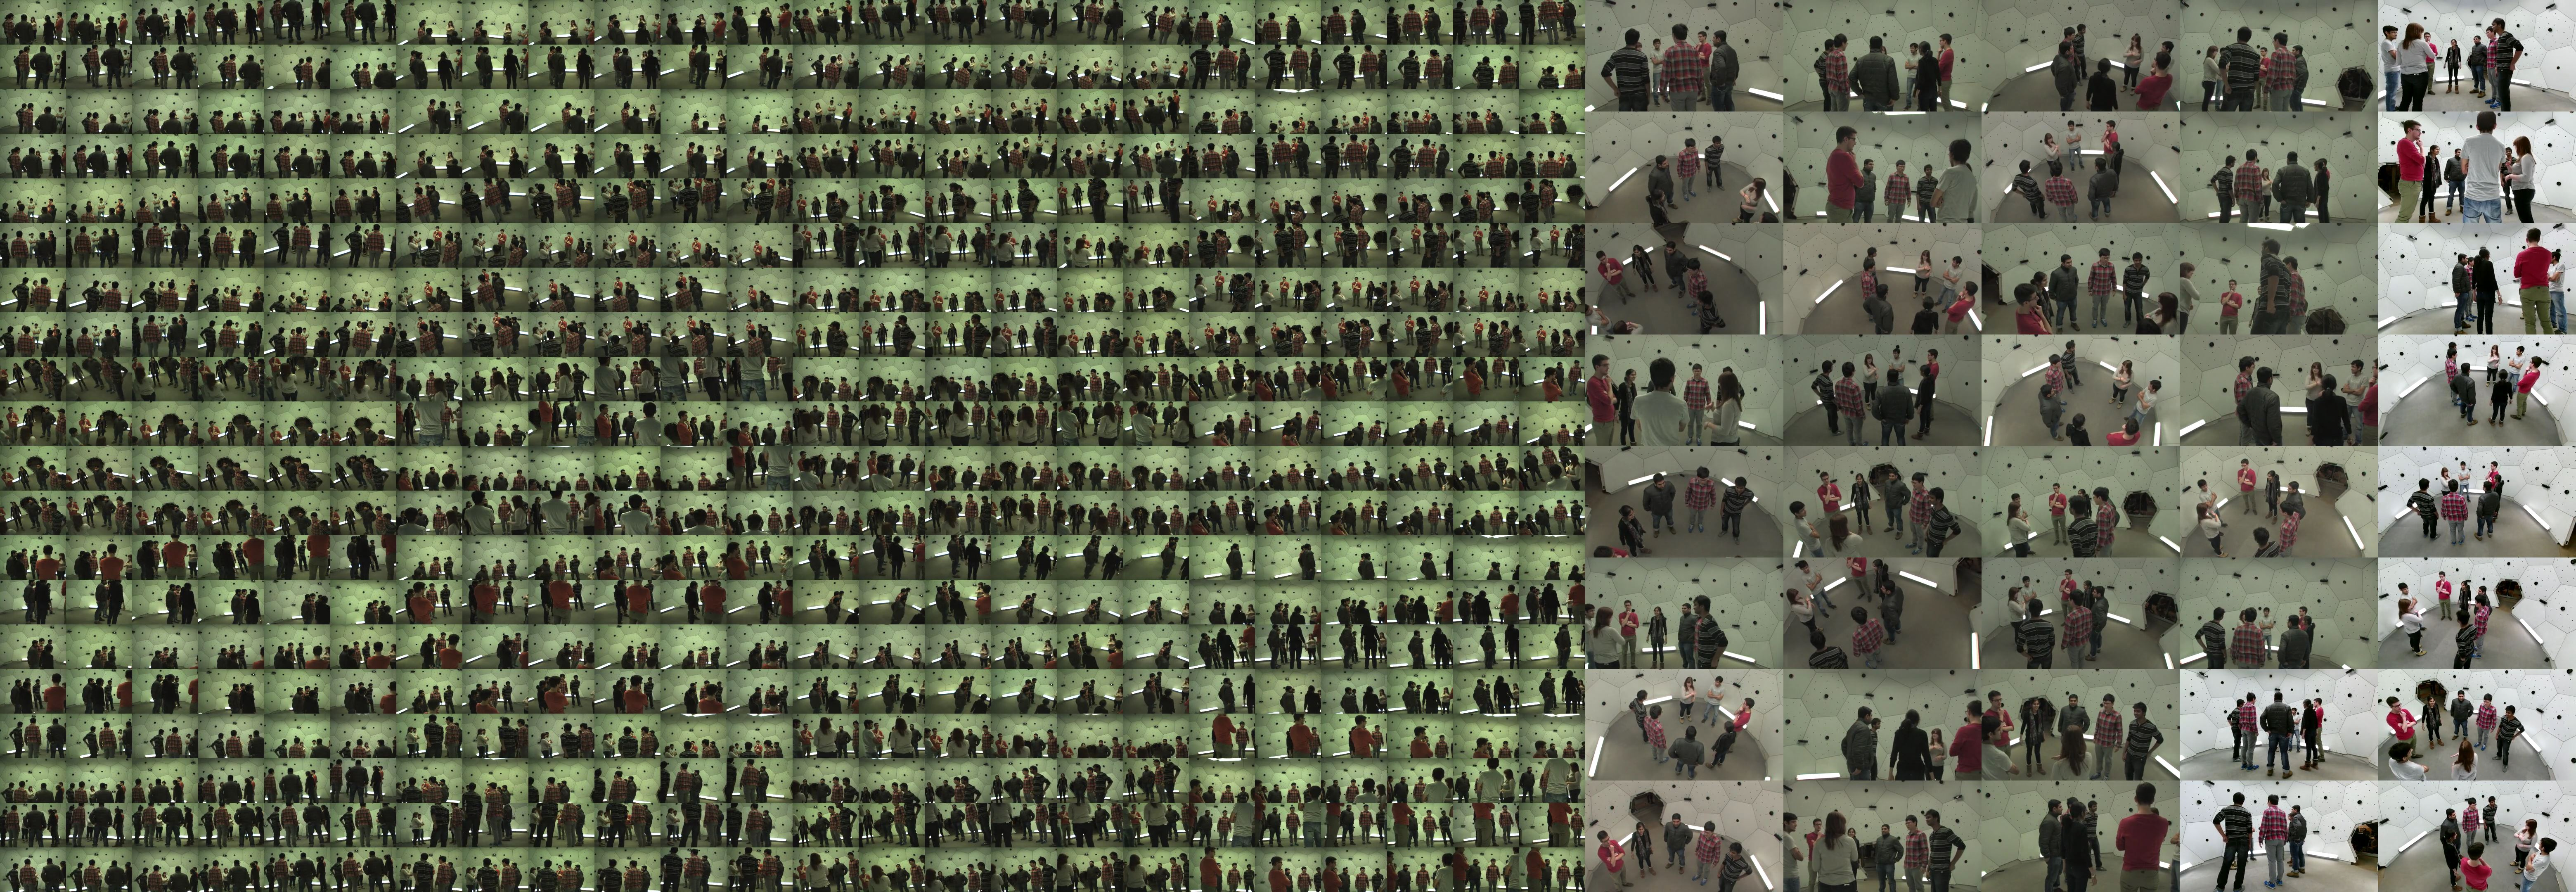
\includegraphics[trim=0 0 0 0,clip,width=\linewidth]{figures/Teaser}
	\includegraphics[trim=0 0 0 0,clip,width=\linewidth]{fig_system/480views_1126}
	\caption{An example scene from 520 camera views of the Panoptic Studio, from 480 VGA cameras, 30 HD cameras, and 10 RGB cameras of the RGB+D sensors.}
	\label{fig:dome_exampleScene}
\end{figure}

\begin{figure}
	\centering       
	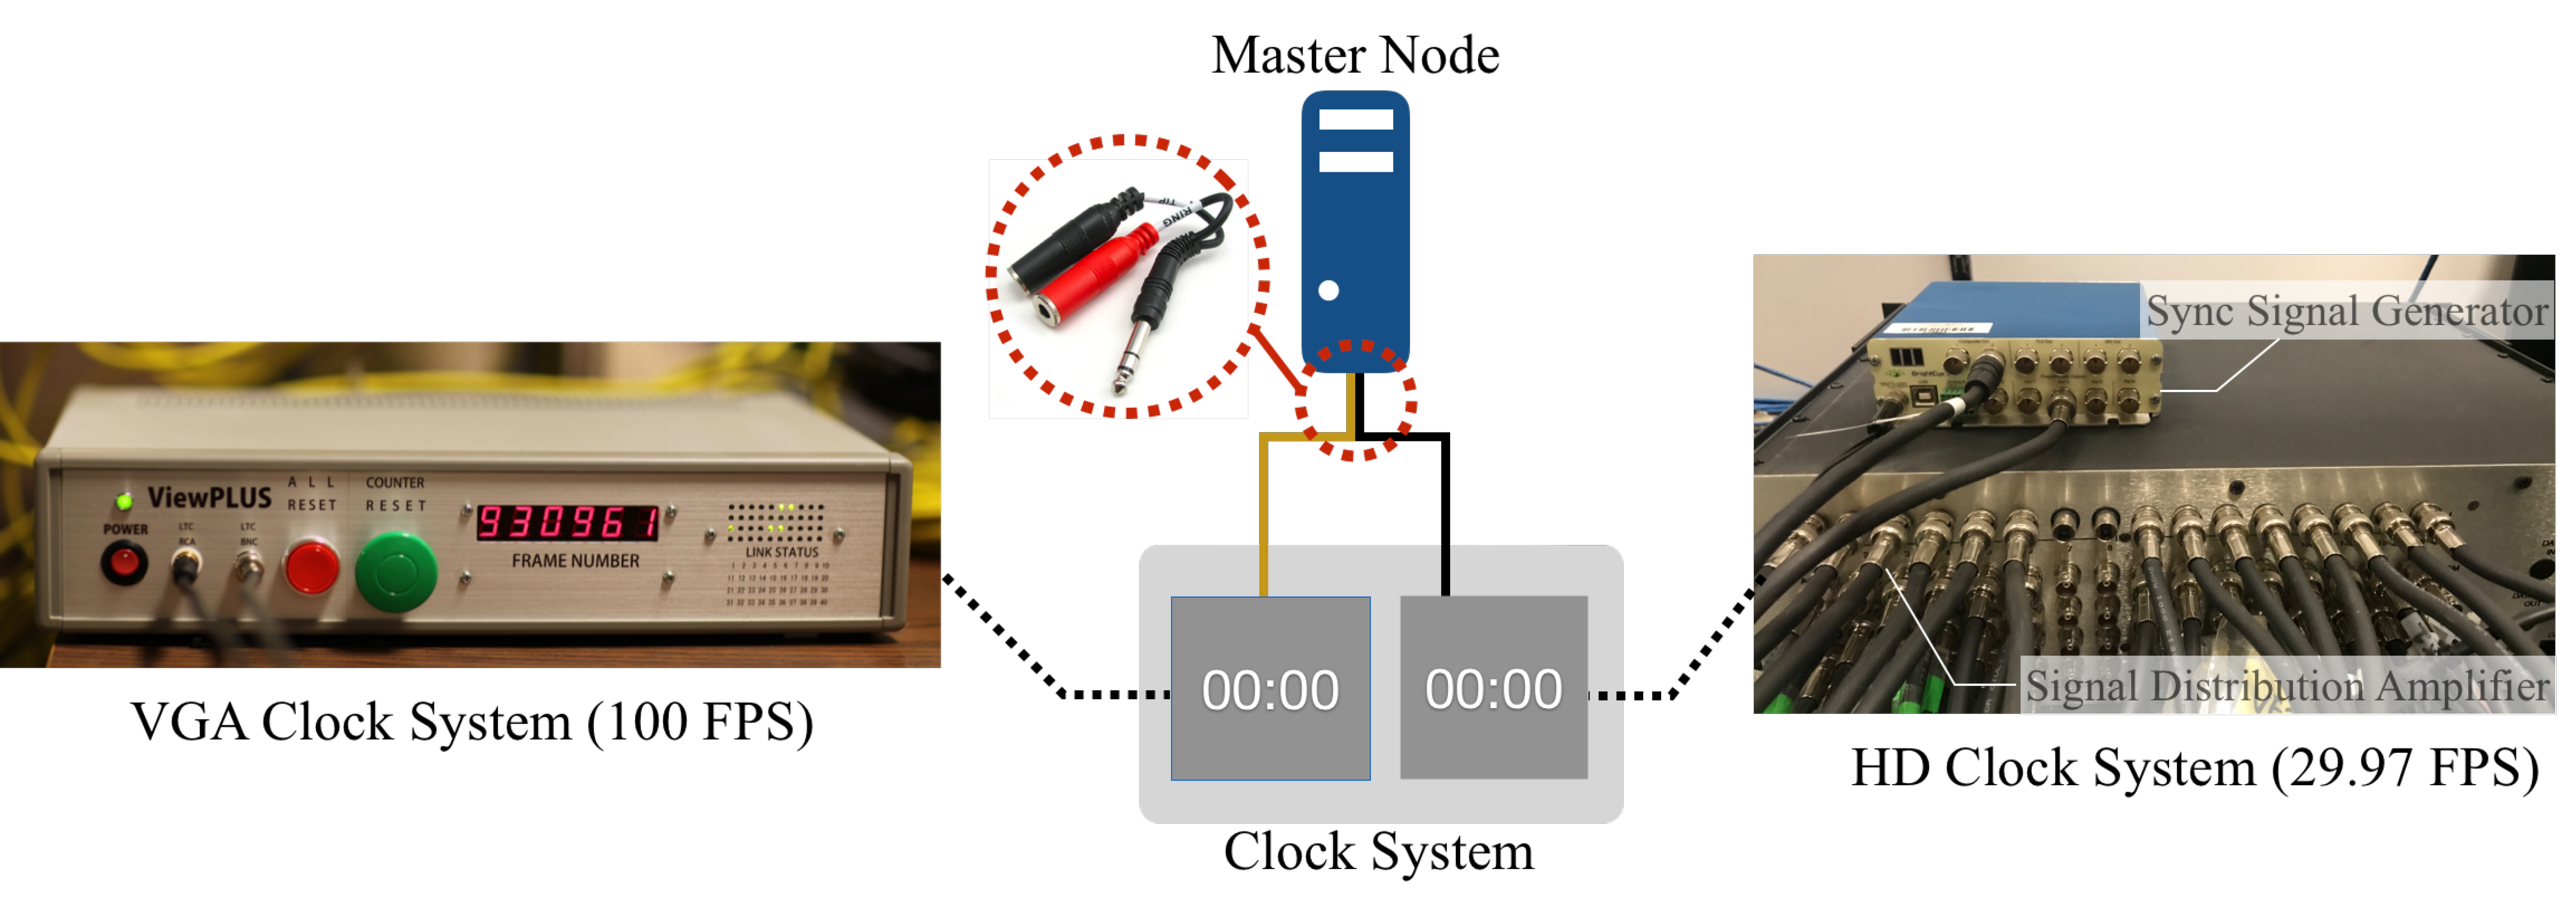
\includegraphics[trim=0 0 0 0,clip,width=\linewidth]{fig_system/dome_syncSystem}
	\caption{Time alignment between VGA camera system and HD camera system. The VGA clock generates 100 Hz time signals, which is downsampled to 25 Hz in VGA cameras, while the HD clock generates signals in 29.97 Hz. We connect them as a stereo audio signal and record it during the capture, which can be decoded afterward for temporal alignment.}
	\label{fig:dome_syncSystem}
\end{figure}
\mbox{ }\\
%The 31 HD cameras are installed at the center of each panel, and 
\noindent \textbf{HD Camera System:} HD cameras are also modularized and each pair of cameras are connected to a local node machine via SDI cables. We use Cannon XH G1s High Definition camcorders, each of which has 3 CCD sensors and captures scenes at 29.97 Hz with ($1920{\times}1080$) resolution. Each HD camera is equipped with a Canon 4.5-90 mm f1.6-f3.5 HD resolving lens, which we fit with a wide angle converter (Canon WD-H72). All HD cameras are genlocked and time-coded, driven by an external clock. The details of the HD camera modules are shown in Figure~\ref{fig:dome_hdSystem}. The data from a pair of HD cameras is transferred via HD-SDI to a local HD node. Each local node saves the data from two cameras to two SSD storage units respectively. 16 HD nodes are dedicated for 31 HD cameras, as shown in the right of the Figure~\ref{fig:dome_machines}.

%Additionally, a total of 10 Kinect v2 RGB+D sensors are mounted at heights of 1m and 2.6 meters, forming two rings with 5 evenly spaced sensors each. 
\mbox{ }\\
\noindent \textbf{RGB+D Sensor System:} Each RGB+D sensor is connected to a dedicated capture node that is mounted on the dome exterior. To capture at rates of approximately 30 Hz, the nodes are equipped with two SSD drives each and store color, depth, and infrared frames as well as body and face detections from the Kinect SDK. A separate master node controls and coordinates the 10 capture nodes via the local network. The details of this subsystem are described in the thesis work of Simon~\cite{simon2017}.

\mbox{ }\\
\noindent \textbf{Data Size and Storage System:} The data size of a minute of data from entire sensors is about 531 GB. The detailed data size for each sub-system is summarized in Figure~\ref{fig:dome_datasize} and an example scene captured by all the sensors are shown in the Figure~\ref{fig:dome_exampleScene}. The data from each sensor module is first saved to a local storage system in each connected node. We use different local storage solutions based on the data size generated by each sensor type. For VGA module with 25 cameras, we use 3 HDDs integrated as RAID-0. This solution provides fast writing speed with a sufficient storage size to store more than two hours of data with relatively low cost\footnote{However, as known, the RAID-0 system is unstable with frequent RAID failures.}. For each HD camera, we dedicate a 1TB SSD, which can store more than 2 hours of data. And for Kinect module, we dedicate two 1TB SSDs. All sensor data in the local storages are transferred to NAS for long-term storage, shown in Figure~\ref{fig:dome_NAS}, by a backup script. Currently, the Panoptic Studio system has about 1.5 PB long-term storage space.


%\begin{figure}
%	\centering       
%	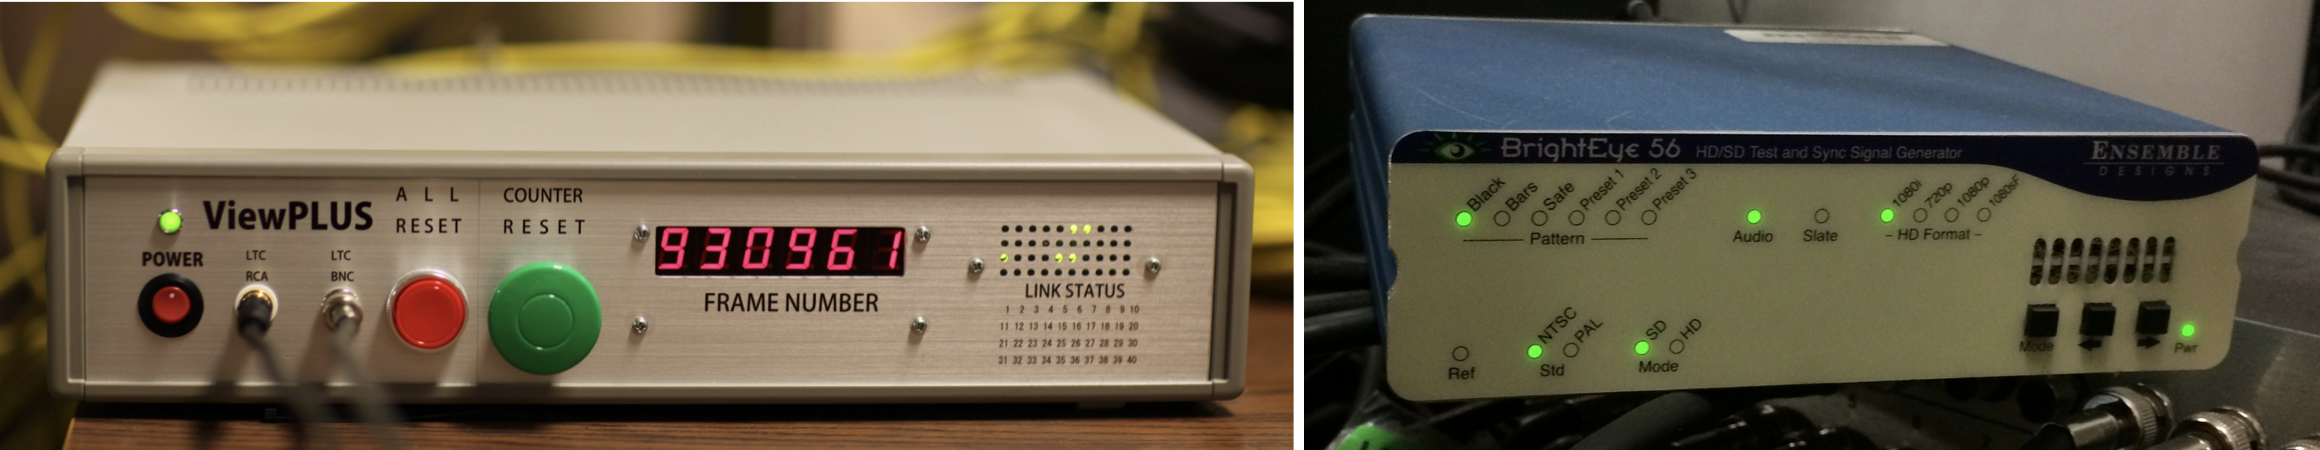
\includegraphics[trim=0 0 0 0,clip,width=\linewidth]{fig_system/dome_syncgens.png}
%	\caption{Sync generators.} 
%\end{figure}

\begin{figure}
	\centering
	%	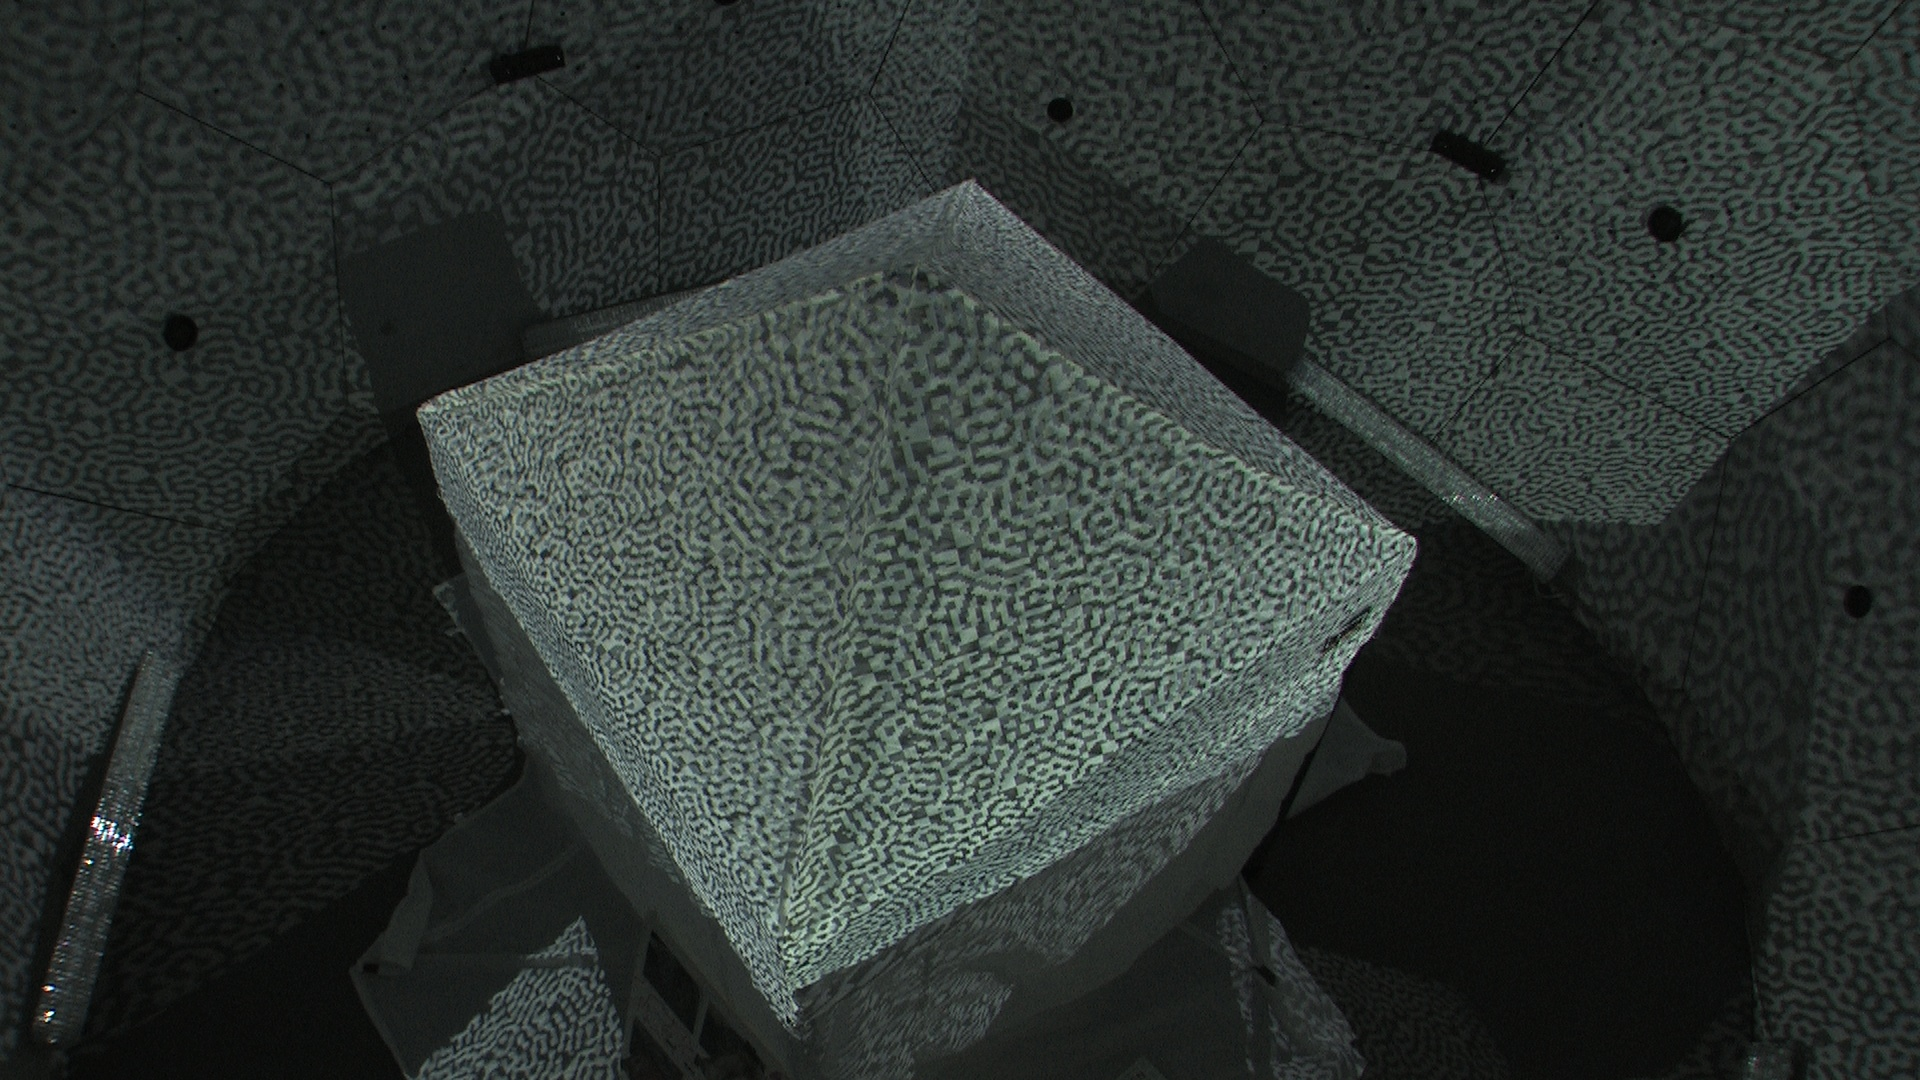
\includegraphics[height=0.2\linewidth]{figures/calib_tent_hd}
	%	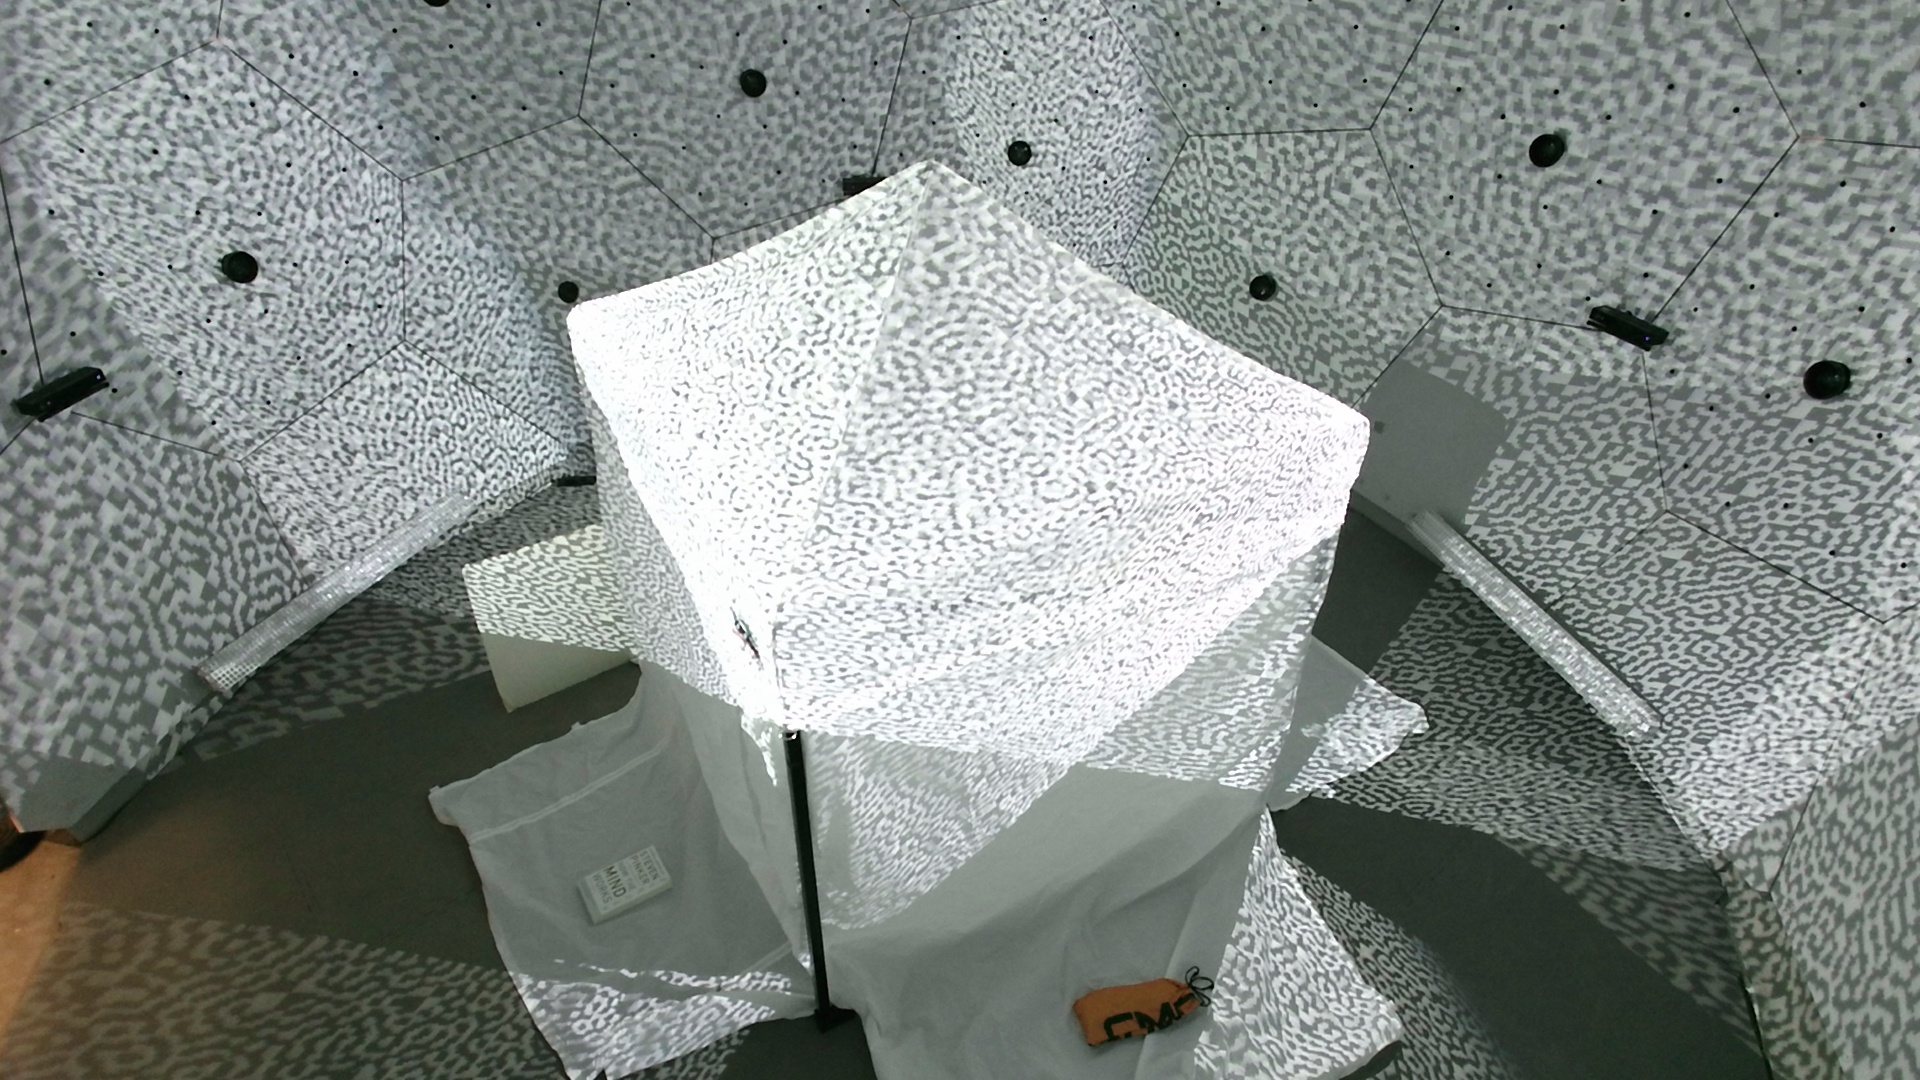
\includegraphics[height=0.2\linewidth]{figures/calib_tent_kinect}
	%	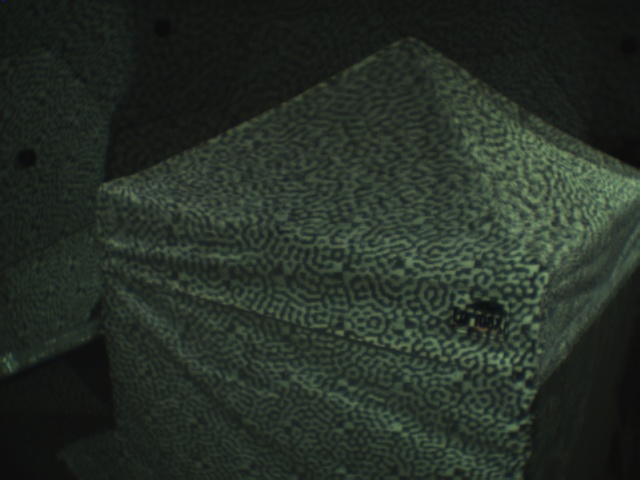
\includegraphics[height=0.2\linewidth]{figures/calib_tent_vga}\\
	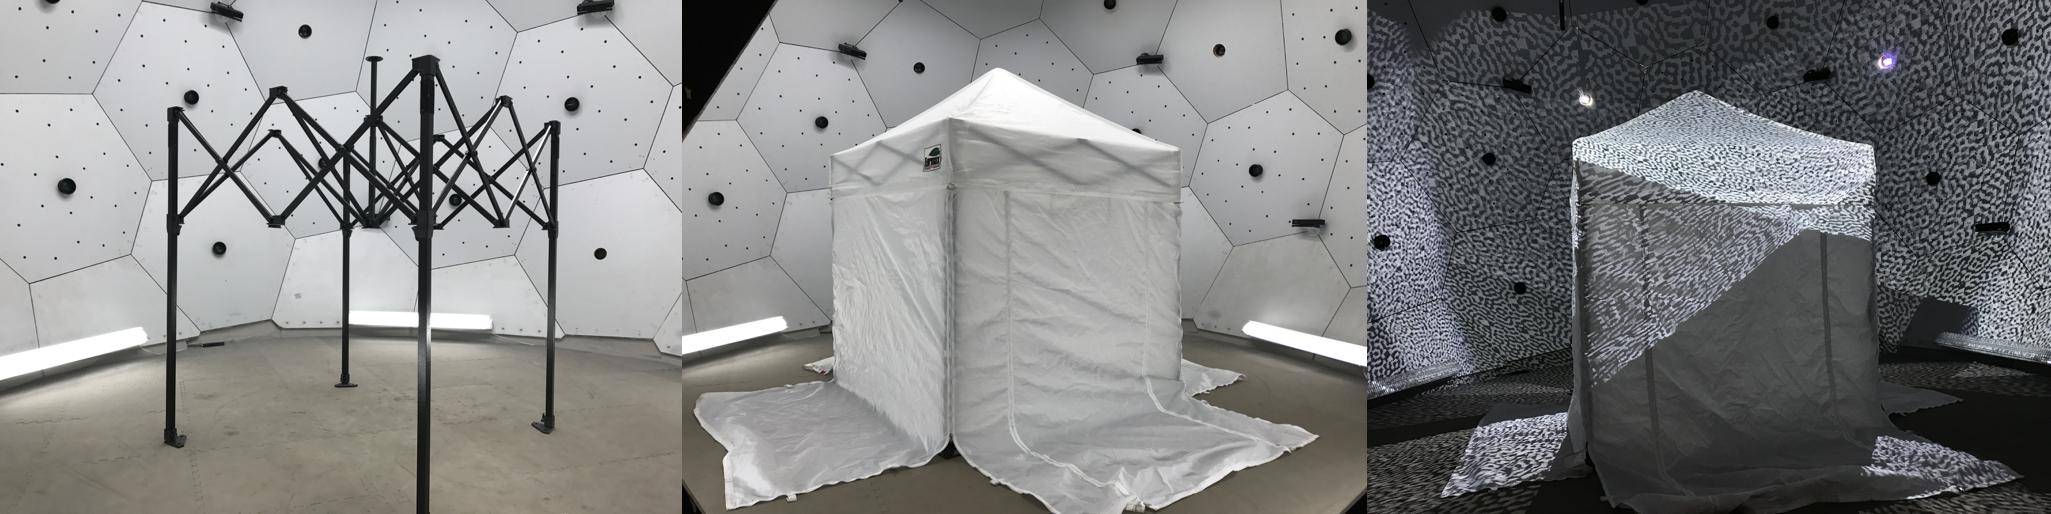
\includegraphics[width=\linewidth]{fig_system/cali_tent_3rdViews}\\
	\vspace{0.2cm}
	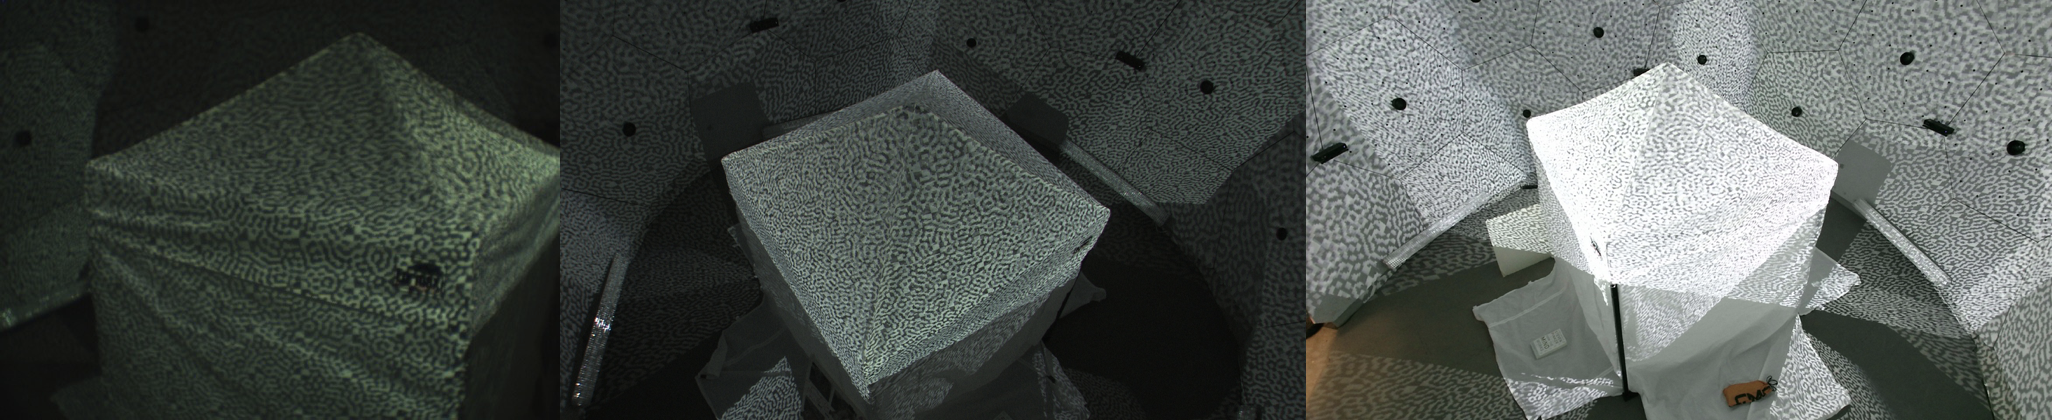
\includegraphics[width=\linewidth]{fig_system/cali_tent_camViews}\\
	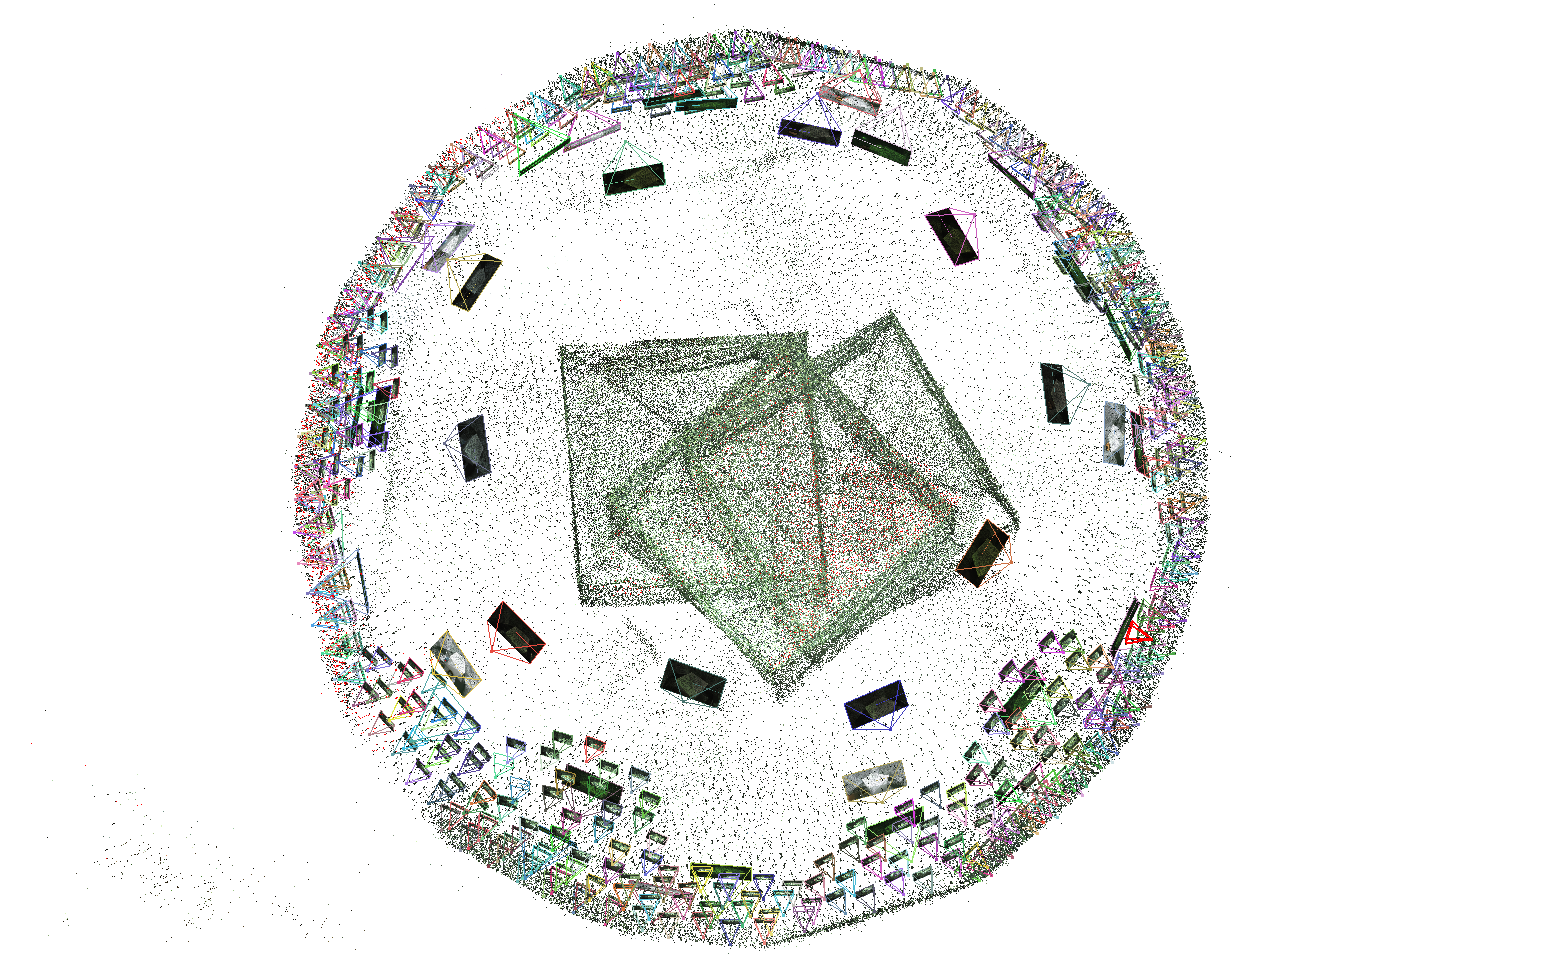
\includegraphics[trim=70 0 70 0,clip,width=0.45\columnwidth]{figures/domeCalib/38}  
	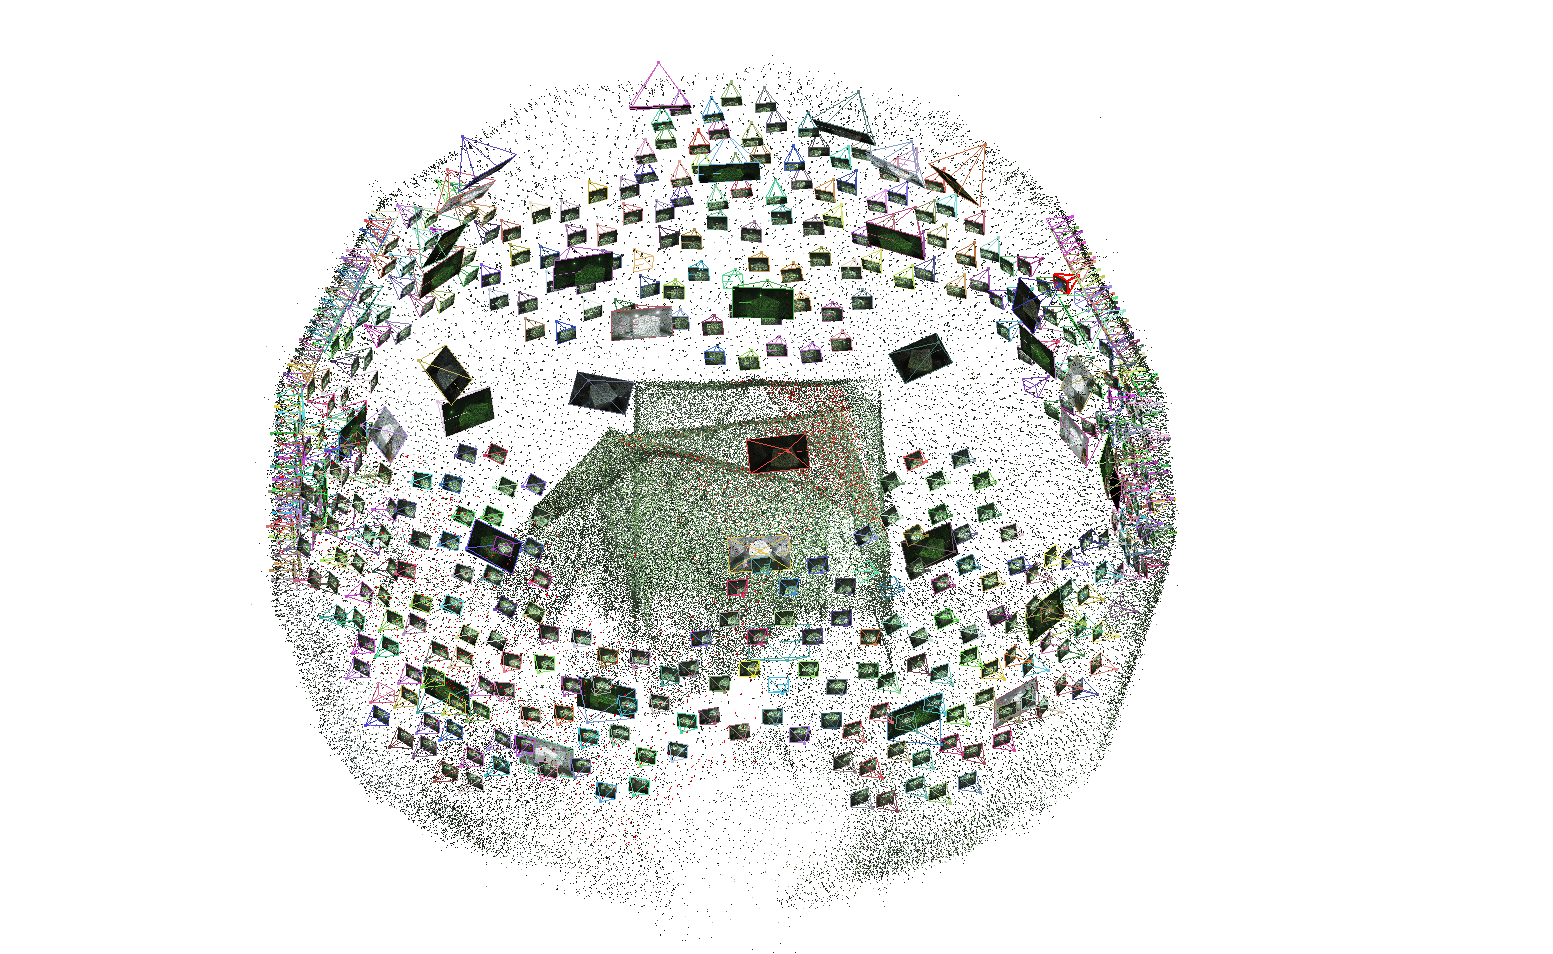
\includegraphics[trim=60 0 80 0,clip,width=0.45\columnwidth]{figures/domeCalib/39}  
	\caption{For efficient spatial calibration process, we use a portable folding tent structure by projecting random patterns from 5 DLP projectors. (Top row) the portable tent and projected patterns; (Middle left) a VGA view; (Middle center) an HD view; (Middle right) a Kinect view from its color camera; (Bottom row) Visualizations of 3D camera localization and a reconstructed 3D point cloud.} 
	\label{fig:spatialCalibration}
\end{figure}

\section{Temporal Calibration for Heterogeneous Sensors}
Synchronizing the cameras is necessary to use geometric constraints (such as triangulation) across multiple views. In our system, we use hardware clocks to trigger cameras at the same time. Because the frame rates of the VGA and HD cameras are different (25 fps and 29.97 fps respectively) we use two separate hardware clocks to achieve shutter-level synchronization among all VGA cameras and among all HD cameras, respectively. To precisely align both time references, we record the timecode signals generated from the two clocks as a single stereo audio signal, which we then decode to obtain a precise alignment at sub-millisecond accuracy, as shown in Figure~\ref{fig:dome_syncSystem}.

Time alignment with the Kinect v2 streams (RGB and depth) is achieved with a small hardware modification: each Kinect's microphone array is rewired to instead record an LTC timecode signal\footnote{As a result of this modification, microphone output on the Kinects is therefore discarded. More details about this hardware modification are available upon request.}.  This timecode signal is the same that is produced by the genlock and timecode generator used to synchronize the HD cameras, and is distributed to each Kinect via a distribution amplifier. We process the Kinect audio to decode the LTC timecode, yielding temporal alignment between the recorded Kinect data---which is timestamped by the capture API for accurate relative timing between color, depth, and audio frames---and the HD video frames. Empirically, we have confirmed the temporal alignment obtained by this method to be of at least millisecond accuracy.
%, with the RGB sensor being a rolling shutter with a scan time of approximately 25ms.


\section{Spatial Calibration}
We use Structure from Motion (SfM) to calibrate all of the 521 cameras. To effectively generate feature points for SfM, five projectors are also installed on the geodesic dome. For calibration, they project a random pattern on a white structure as shown in the Figure~\ref{fig:spatialCalibration}, and multiple scenes (typically three) are captured by moving the structure within the dome. We perform SfM for each scene separately and perform a bundle adjustment by merging all the matches from each scene. We use a VisualSfM software~\cite{vsfm} with 1 distortion parameter to produce an initial estimate and a set of candidate correspondences, and subsequently run our own bundle adjustment implementation with 5 distortion parameters for the final refinement. The computation time is about 12 hours with 6 scenes (521 images for each) using a 6 core machine. 
In this calibration process, we only use the color cameras of Kinects. We additionally calibrate the transformation between the color and depth sensor for each Kinect with a standard checkerboard pattern, placing all cameras in alignment within a global coordinate frame.
%and the depth cameras are stitched to the global camera coordinate of other cameras in the end. 

\section{Lighting, Audio Recording, and Capture Softwares}

\noindent \textbf{Lighting:} We use a relatively low-cost solution for lighting by installing fluorescent lamps on the ceiling and floors, as shown in Figure~\ref{fig:dome_lighting}. The floor lights are important to reduce the shadow issues of the scenes. 
\mbox{ }\\
\noindent \textbf{Audio Recording:} Audio from microphones can be easily recorded and synchronized with cameras by connecting microphones to HD cameras. Each HD camera has two mono microphone inputs, by which the audio signals are saved as a stereo audio file. We installed one microphone on the floor and two microphones on the ceiling. We also use 20 wireless lapel microphones by connecting the wireless receivers to HD cameras, as shown in Figure~\ref{fig:dome_mic}. Each lapel microphone is assigned to a subject during the social interaction capture.  
\mbox{ }\\
\noindent \textbf{Capture Softwares:} As an important part of the system, we built several custom software systems to control the capture process. Each subsystem is controlled by a separate capture software. We built a shell script to initiate both VGA and  HD capture software along with the sync signal recording together in the master node. For VGA, we built a server-client software system, where a local server is opened and runs at each VGA node to communicate with the master node. In the master node, an operator can check the status of each VGA module, visualize the camera views in real-time streaming, and initiate the capture. The VGA capture tool is shown in the Figure~\ref{fig:dome_vgaSW}. For the HD, we use a secure shell (SSH) protocol to automatically initiate the capture software at each machine. Kinect is separately controlled by the Kinect master node.

After the capture, the captured scenes from VGA and HD sensors can be visualized in our viewer, as shown in Figure~\ref{fig:dome_viewer}, where the viewer loads capture data by remotely connecting all local storages. 

\begin{figure}
	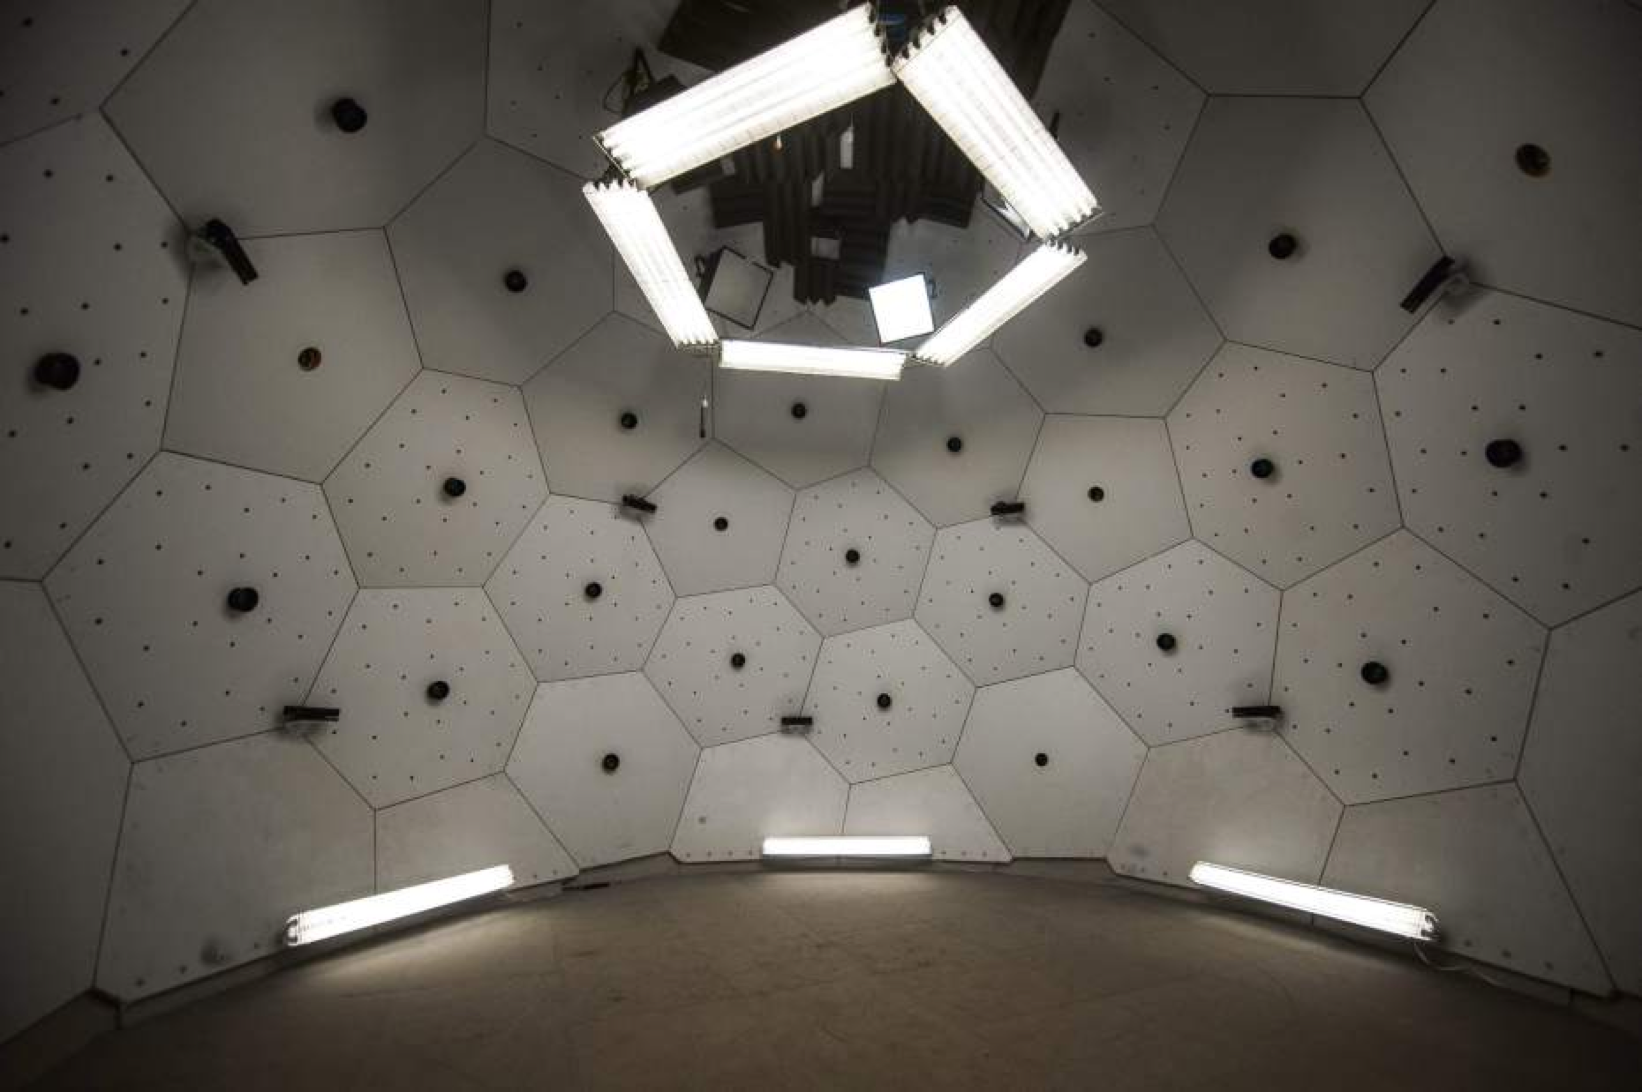
\includegraphics[width=\linewidth]{fig_system/dome_lighting}
	\caption{We use a relatively low-cost solution for lighting by installing fluorescent lamps on the ceiling and the floor.}
	\label{fig:dome_lighting}
\end{figure}

\begin{figure}
	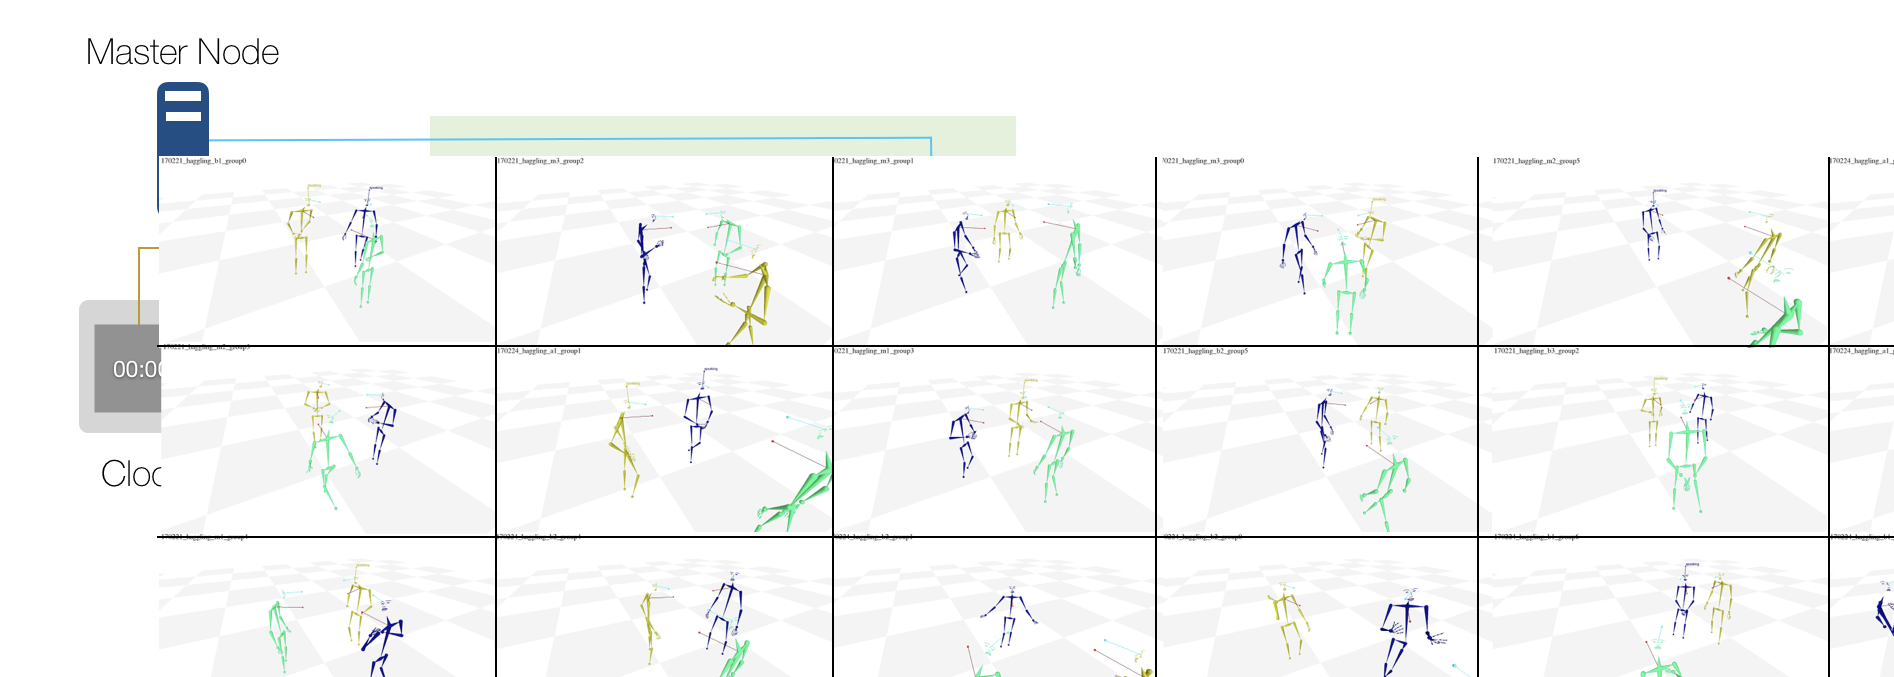
\includegraphics[width=\linewidth]{fig_system/dome_mic}
	\caption{Each HD camera has two mono microphone inputs, by which the audio signals are saved as a stereo audio file. We also use 20 wireless lapel microphones by connecting the wireless receivers to HD cameras.}
	\label{fig:dome_mic}
\end{figure}

\begin{figure}
	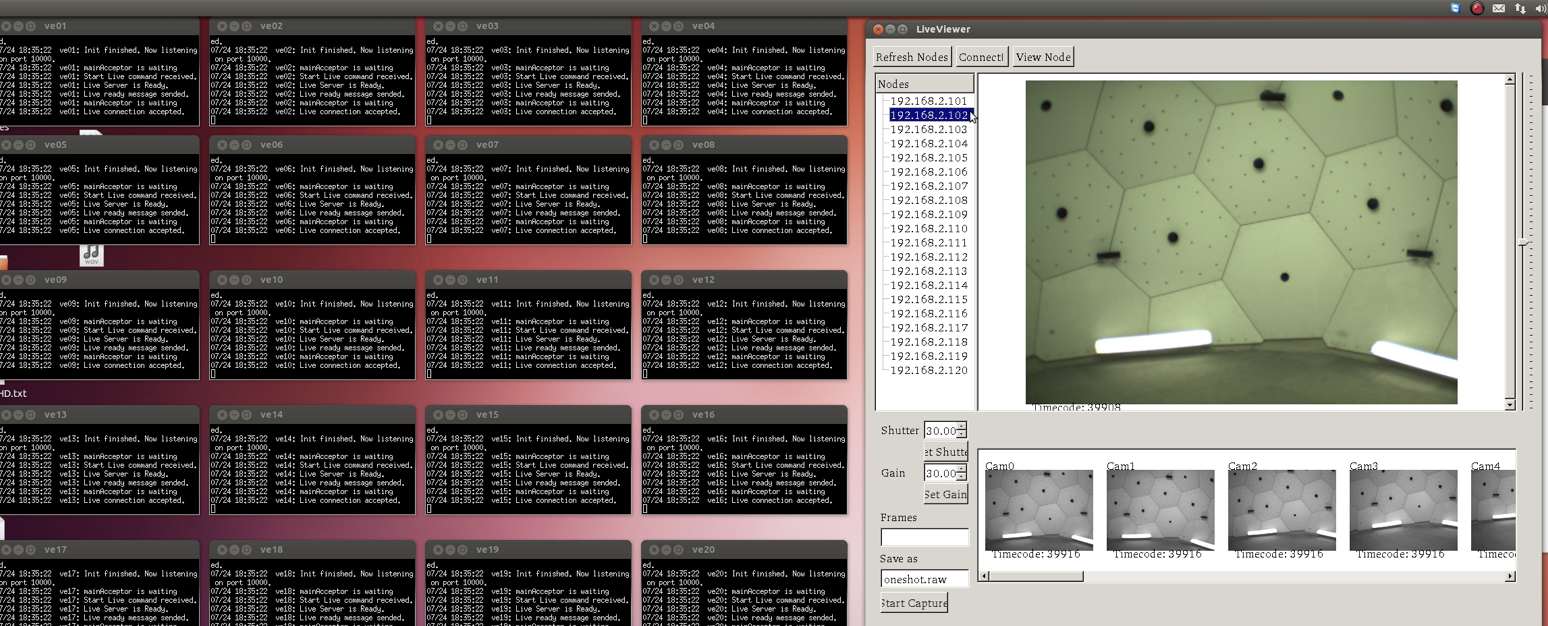
\includegraphics[width=\linewidth]{fig_system/dome_sw_capture.png}
	\caption{A capture software for VGA sub-system. In the master node, users can check the status of each VGA module (black consoles on the left), visualize the camera views in real-time streaming (the GUI tool on the right), and initiate the capture.}
	\label{fig:dome_vgaSW}
\end{figure}\vspace{0.5cm}
	
\begin{figure}[t]
	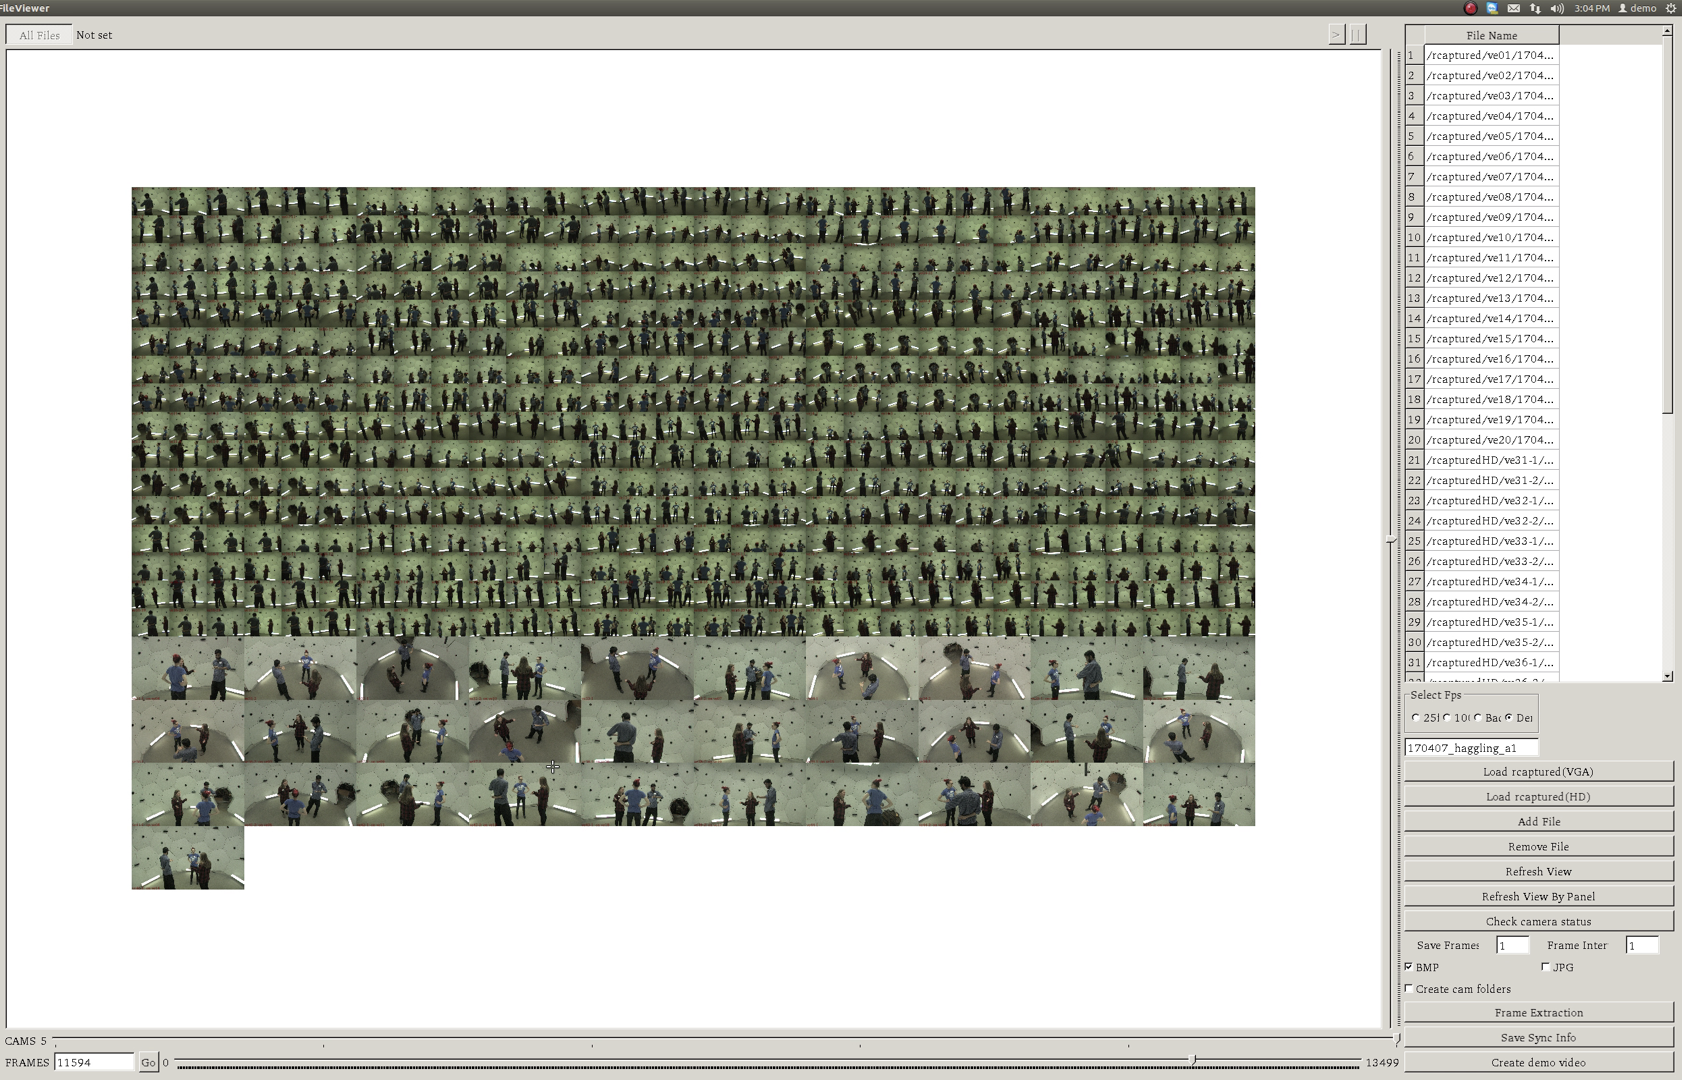
\includegraphics[width=\textwidth]{fig_system/dome_sw_viewer.png}
	\caption{A viewer to visualize the captured data from VGA and HD cameras.}
	\label{fig:dome_viewer}
	%\caption{Panoptic Studio Software System}
\end{figure}

\section{Discussion}
We found three limitations in our hardware design which can be reconsidered for follow-up research. The first is the incompatible frame rates among heterogeneous sensors, especially between HD cameras and VGA cameras, which makes it hard to fuse them for 3D reconstruction. Due to this reason, we use each subsystem for different purposes; The VGA system is mainly used to reconstruct 3D body motions, and HD system is used to reconstruct the face and hand motions. In the end, all reconstruction results are combined via an interpolation. A better synchronization may enable much easier solutions to leverage all sensors together. The second issue is that all the camera views mainly focus on the center of the dome and, thus, fewer views are available at the edges of the capture volume. Such design is ideal given the assumption that subjects are located at the center of the system, but we observe that sometimes people tend to stand near the walls during social interactions. An alternative direction would be to make cameras focus on random locations so that view coverage can be uniformly spread throughout the working volume. Last, we found that the spatial and temporal resolutions of cameras installed in the studio limit the reconstruction quality. Sensors with higher resolution and faster speed need to be considered in the follow-up research.

%\section{Lighting}
%\section{Storage}
%\section{Hardware Details}
%\section{Capture Procedures}
%\section{Data Size}

%We use projectors to generate patterns. 
%We turn on projector one by one to reduce interference among them. 
%We run SfM using all the data. 
%We merge all the matching into a whole optimization. 
%
%With/Without tent
%All projectors/each projectors
%1 tent location, several tent location
%
%We evaluate the accuracy using a single scene with 2D maching points. Using each calibration, we reconstruct 3D and compute reprojection  error. 
%We use leave-out method to check each camera's reprojection error. 
%For kinect, we use checker board pattern. 
%Temporal alignment
%Among VGA
%Among HD
%Among Kinect
%VGA-HD
%VGA-HD-Kinect




\pagebreak